\documentclass[a4paper]{ctexart}
\usepackage[top=3cm, bottom=2cm]{geometry}
\usepackage{graphicx}
\graphicspath{{fig/}}
\usepackage{subcaption}
\usepackage{amsmath}
\usepackage{amssymb}
\usepackage{xcolor}
\usepackage{url}
\usepackage{booktabs}
\usepackage{multirow}
%\usepackage{hyperref}
\usepackage[hidelinks]{hyperref} % 加载 hyperref 并隐藏链接边框

%\usepackage[utf8]{inputenc}
%\usepackage[ngerman]{babel} % 加载德语支持

% booktabs 提供 \toprule, \midrule, \bottomrule 等表格命令
% (booktabs 已在第9行加载，此处不再重复)

% 定义占位命令以避免未定义控制序列错误
%\newcommand{\placeholderspace}{}
\usepackage{fancyhdr} % 导入fancyhdr宏包
\usepackage{lipsum}   % 仅用于生成示例文本
\usepackage{float}    % 提供 H 浮动位置选项


\pagestyle{fancy}
\fancyhead[L]{}
\fancyhead[C]{\textbf{Physics-experiment Reporting Letter:\\Spin Dynamics of Quantum Materials}}
\fancyhead[R]{}
\fancyfoot[L]{}
\fancyfoot[C]{\thepage}
\fancyfoot[R]{}
\renewcommand{\headrulewidth}{1.4pt}
\renewcommand{\footrulewidth}{0pt}
\setlength{\headheight}{24pt}
\setlength{\emergencystretch}{3em}

\title{量子材料的自旋动力学虚拟仿真实验}
\author{实验人：学生\qquad 学号：[学号已脱敏]}
\date{实验日期：2026.6.18}

\begin{document}

\maketitle

\begin{abstract}
本实验通过虚拟仿真平台学习量子材料自旋动力学及中子散射谱学测量方法。实验内容包括预习与安全学习、金刚石声子谱测量以及铁基超导母体材料 BaFe$_2$As$_2$ 自旋波谱测量三个部分。通过预习模块，理解中子散射能够同时获得动量转移和能量转移信息，因而适合研究晶格振动与磁激发；通过金刚石模块，利用三轴谱仪完成弹性散射定向，并在非弹性散射模式下沿高对称方向得到声学支和光学支声子谱；通过 BaFe$_2$As$_2$ 模块，在低于结构相变温度 $T_S\approx138\,\mathrm{K}$ 和磁相变温度 $T_N\approx137\,\mathrm{K}$ 的条件下，利用飞行时间谱仪观察不同能量窗口中的自旋激发分布。

实验结果表明，弹性散射适合确定晶体取向，非弹性散射可用于研究声子、自旋波等动态激发。金刚石沿 [100] 高对称方向的声子谱中可分辨 TA、LA、TO、LO 四支主要分支；BaFe$_2$As$_2$ 在低能窗口 $E=[58,64]\,\mathrm{meV}$ 附近表现出反铁磁波矢附近的自旋激发强度集中，高能窗口 $E=[213,234]\,\mathrm{meV}$ 进一步反映自旋激发的对称性与能量依赖性。本实验还强调了低温、真空、液氦回收和辐射剂量检测等安全规范在大型中子实验中的必要性。

\textbf{关键词：量子材料\quad 自旋动力学\quad 中子散射\quad 声子谱\quad 自旋波}
\end{abstract}

\section{引言}

量子材料是指其宏观性质显著受量子效应、电子关联、自旋自由度和晶格自由度共同影响的一类材料。高温超导、量子反常霍尔效应、低维磁性和拓扑物态等现象都说明，材料的电学、磁学和热学性质不能仅从经典图像出发理解。对于许多量子材料而言，晶格振动与磁相互作用会共同决定低能激发谱，并进一步影响相变、输运和超导配对等物理过程。

自旋动力学研究磁矩随时间和空间的集体变化。若材料中存在长程磁有序，外界扰动可激发磁矩围绕平衡方向进动，形成自旋波；若材料处于强磁涨落状态，自旋关联仍可能在能量--动量空间中表现为可测的谱强度。因而，测量自旋激发的能量、动量分布和各向异性，是理解量子材料磁相互作用的重要途径。

中子散射是研究晶体结构、声子和磁激发的重要实验手段。中子不带电，穿透性强；同时中子具有磁矩，可以与电子自旋产生磁相互作用。与普通光学实验相比，中子散射能够通过散射前后的波矢和能量变化直接给出动量转移 $\mathbf{Q}$ 与能量转移 $E$，因此特别适合研究声子色散和自旋波谱。本虚拟仿真实验以三轴谱仪和飞行时间谱仪为主要实验平台，通过金刚石声子谱和 BaFe$_2$As$_2$ 自旋波谱两个案例，建立从仪器参数设置到物理图像分析的完整认识。

\section{实验目的}

\begin{enumerate}
    \item 了解量子材料中晶格振动、磁相互作用和自旋激发的基本物理图像。
    \item 理解中子散射在研究量子材料中的作用，掌握动量转移、能量转移和散射强度之间的关系。
    \item 掌握三轴谱仪与飞行时间谱仪的基本测量思路，区分弹性散射和非弹性散射的典型应用。
    \item 通过金刚石声子谱测量，理解样品定向、能量扫描和声子分支识别方法。
    \item 通过 BaFe$_2$As$_2$ 自旋波谱测量，认识磁有序态中自旋激发的能量依赖性和空间分布特征。
    \item 熟悉低温、真空、液氦回收和辐射剂量检测等大型中子实验中的安全规范。
\end{enumerate}

\section{实验原理}

\subsection{中子散射中的动量转移与能量转移}

设入射中子波矢和能量分别为 $\mathbf{k_i}$、$E_i$，出射中子波矢和能量分别为 $\mathbf{k_f}$、$E_f$。散射过程中的动量转移和能量转移可写为
\begin{equation}
    \mathbf{Q}=\mathbf{k_i}-\mathbf{k_f},
\end{equation}
\begin{equation}
    E=\hbar\omega=E_i-E_f .
\end{equation}
若 $E=0$，中子只改变运动方向而不与样品交换能量，该过程称为弹性散射，常用于测定晶体结构和样品取向。若 $E\neq0$，中子与样品中的集体激发交换能量，该过程称为非弹性散射，可用于测量声子、自旋波等动态过程。

中子的德布罗意关系为
\begin{equation}
    E=\frac{\hbar^2 k^2}{2m_n},
\end{equation}
其中 $m_n$ 为中子质量。通过选择入射或出射中子的能量，并测量散射角，就可以确定实验所对应的倒易空间位置与能量转移。

\subsection{三轴谱仪}

三轴谱仪通常由单色器、样品台和分析器三部分构成，对应三个可转动的主要轴。单色器从白中子束中选择特定入射能量，样品台控制晶体取向，分析器选择特定出射能量。三轴谱仪的特点是能量和动量分辨率较高，适合在倒易空间中逐点扫描。

在弹性散射定向时，入射中子和出射中子能量相同，晶体满足布拉格条件
\begin{equation}
    2d\sin\theta = n\lambda .
\end{equation}
通过扫描样品角并寻找 Bragg 峰，可以建立晶体倒易空间方向与仪器角度之间的对应关系。在非弹性散射测量中，固定或选择某一出射能量 $E_f$，再改变入射能量或散射角，即可在指定 $\mathbf{Q}$ 点附近测量激发能量。

\subsection{飞行时间谱仪}

飞行时间谱仪利用中子从样品到探测器的飞行时间来反推出出射能量。入射中子束经过斩波器后形成脉冲束，若中子飞行路径长度为 $L$，飞行时间为 $t$，则其速度和能量满足
\begin{equation}
    v=\frac{L}{t},
\end{equation}
\begin{equation}
    E=\frac{1}{2}m_n v^2 .
\end{equation}
与三轴谱仪逐点扫描不同，飞行时间谱仪配合大面积探测器阵列，可以在一次测量中覆盖较宽的能量--动量空间，适合观察自旋激发的整体谱图、高能色散和各向异性。

\subsection{声子与声子谱}

晶体中原子围绕平衡位置作集体振动，其量子化激发称为声子。对于含有多个原子的基元，声子分支通常可分为声学支和光学支。声学支在长波极限下对应晶胞整体平移，频率趋近于零；光学支对应基元内不同原子的相对振动，通常具有较高能量。

金刚石具有高度对称的立方晶体结构。沿高对称 [100] 方向测量时，由于横波模式简并，实际可分辨的主要声子分支包括横声学支 TA、纵声学支 LA、横光学支 TO 和纵光学支 LO。实验中沿不同倒易空间方向扫描，可以选择性观察纵波或横波声子。

\subsection{自旋波与 BaFe$_2$As$_2$}

在磁有序材料中，局域磁矩之间的交换相互作用使自旋趋向某种有序排列。若某个自旋受到微扰，扰动会通过交换相互作用在晶格中传播，形成集体激发，即自旋波。自旋波的量子称为磁振子，其能量--动量关系反映了材料中的磁相互作用强度、各向异性和磁有序结构。

BaFe$_2$As$_2$ 是铁基超导体系的重要母体材料。它在降温过程中先经历四方相到正交相的结构相变，随后进入反铁磁有序态，典型相变温度为
\begin{equation}
    T_S\approx138\,\mathrm{K},\qquad T_N\approx137\,\mathrm{K}.
\end{equation}
在低于 $T_N$ 的温区，材料中形成反铁磁有序，因而可以在反铁磁波矢附近观察到自旋波激发。测量不同能量窗口下的散射强度分布，有助于理解铁基超导母体中的磁相互作用和磁涨落特征。

\section{实验内容与步骤}

\subsection{预习与安全学习}

虚拟仿真实验首先通过预习模块建立实验概念。学习内容包括量子材料的典型现象、自旋动力学的研究意义、中子与原子核及电子磁矩的相互作用、三轴谱仪和飞行时间谱仪的工作特点，以及低温样品环境和辐射安全规范。

在安全规范方面，实验特别强调低温、真空和辐射防护。低温恒温器通常包含真空夹层、液氮腔、液氦腔和样品腔，利用多级隔热与低温介质为样品提供稳定测量环境。获得高真空时，需要先使用机械泵粗抽，再使用分子泵进入高真空区间，以避免残余气体影响低温和散射条件。中子实验还要求进行剂量监测、挡板控制和实验结束后的安全检查。

\begin{figure}[H]
    \centering
    \begin{subfigure}[t]{0.48\textwidth}
        \centering
        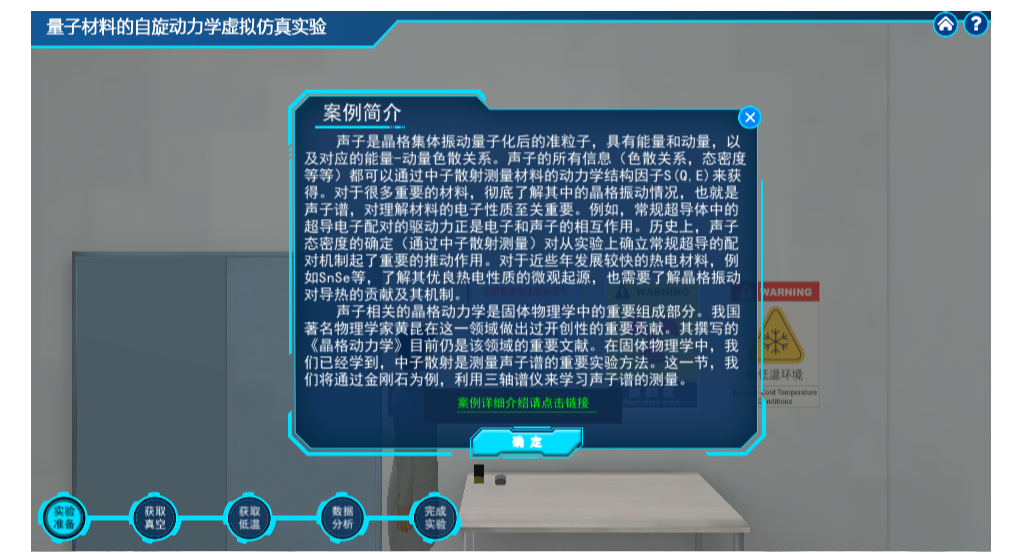
\includegraphics[width=\linewidth]{屏幕截图 2026-06-28 105530.png}
        \caption{案例与实验背景介绍}
    \end{subfigure}
    \hfill
    \begin{subfigure}[t]{0.48\textwidth}
        \centering
        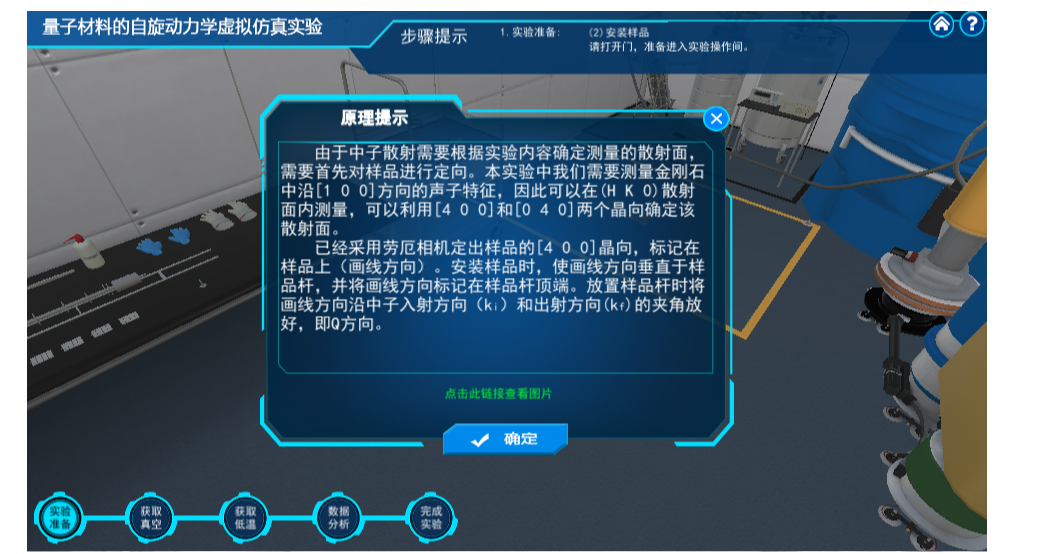
\includegraphics[width=\linewidth]{屏幕截图 2026-06-28 105615.png}
        \caption{中子散射原理学习界面}
    \end{subfigure}
    \caption{虚拟仿真实验的预习与原理学习模块}
    \label{fig:prestudy}
\end{figure}

\subsection{金刚石声子谱测量}

金刚石模块使用三轴谱仪完成。实验先在弹性散射模式下寻找金刚石的 Bragg 点，例如 $(4,0,0)$ 和 $(0,4,0)$，由此确定 $(HK0)$ 散射面。完成初步定向后，继续调整样品角 $\psi$，使扫描曲线峰位与预期位置一致，从而精确建立样品倒易空间坐标和仪器角度之间的关系。

样品定向完成后，实验切换到非弹性散射模式。在不同 $q$ 点改变能量扫描范围，沿 $[4+q,0,0]$ 方向测量纵波声子，沿 $[4,q,0]$ 方向测量横波声子。通过寻找谱峰位置，可得到金刚石沿高对称 [100] 方向的声子色散关系。

\begin{figure}[H]
    \centering
    \begin{subfigure}[t]{0.48\textwidth}
        \centering
        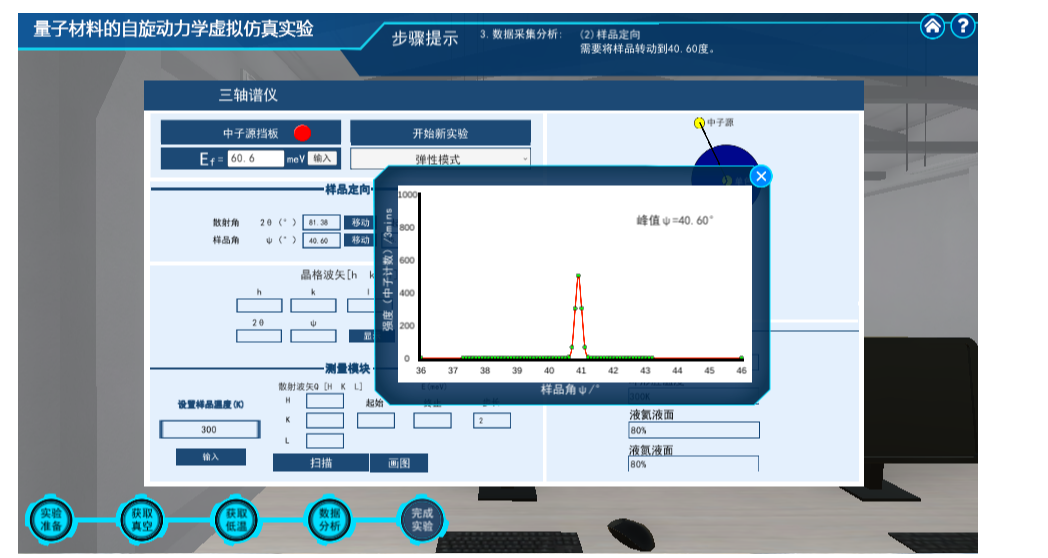
\includegraphics[width=\linewidth]{屏幕截图 2026-06-28 110255.png}
        \caption{第一组弹性散射扫描峰}
    \end{subfigure}
    \hfill
    \begin{subfigure}[t]{0.48\textwidth}
        \centering
        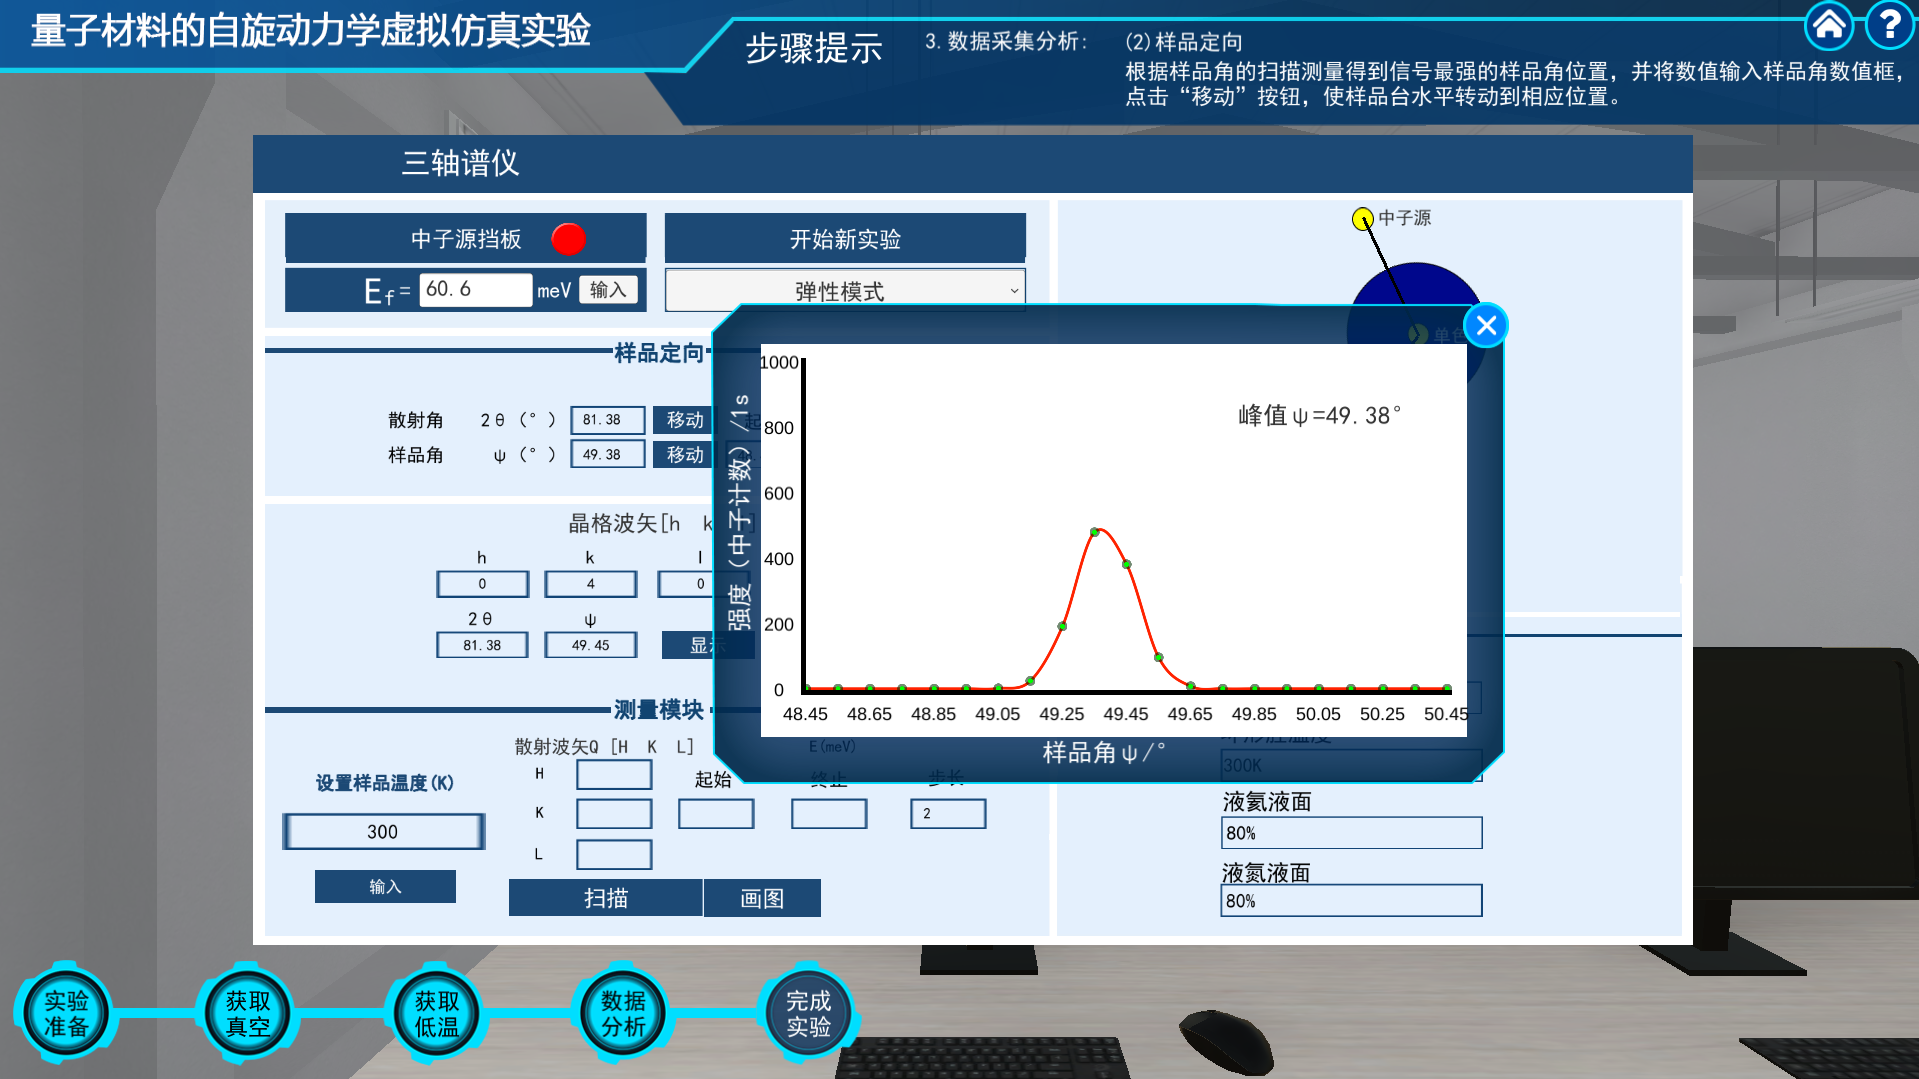
\includegraphics[width=\linewidth]{屏幕截图 2026-06-28 110511.png}
        \caption{调整样品角后的扫描峰}
    \end{subfigure}
    \caption{金刚石样品的 Bragg 峰扫描与取向校准}
    \label{fig:bragg}
\end{figure}

\subsection{BaFe$_2$As$_2$ 自旋波谱测量}

BaFe$_2$As$_2$ 模块使用飞行时间谱仪完成。由于目标是观察反铁磁有序态中的自旋波谱，样品需要降温到低于 $T_S$ 和 $T_N$ 的温区。实验中选择适当的入射中子能量和费米斩波器频率，以获得所需的能量分辨率和动量覆盖范围。

测量时先在较低能量转移窗口中确认反铁磁波矢附近是否存在明显自旋激发，再提高入射能量，观察更高能量范围内自旋激发的空间分布和对称性。虚拟平台给出的典型能量窗口包括低能区
\begin{equation}
    E=[58,64]\,\mathrm{meV},
\end{equation}
以及高能区
\begin{equation}
    E=[213,234]\,\mathrm{meV}.
\end{equation}
通过比较不同能量窗口中的强度图，可以分析自旋激发随能量变化的形态。

\begin{figure}[H]
    \centering
    \begin{subfigure}[t]{0.48\textwidth}
        \centering
        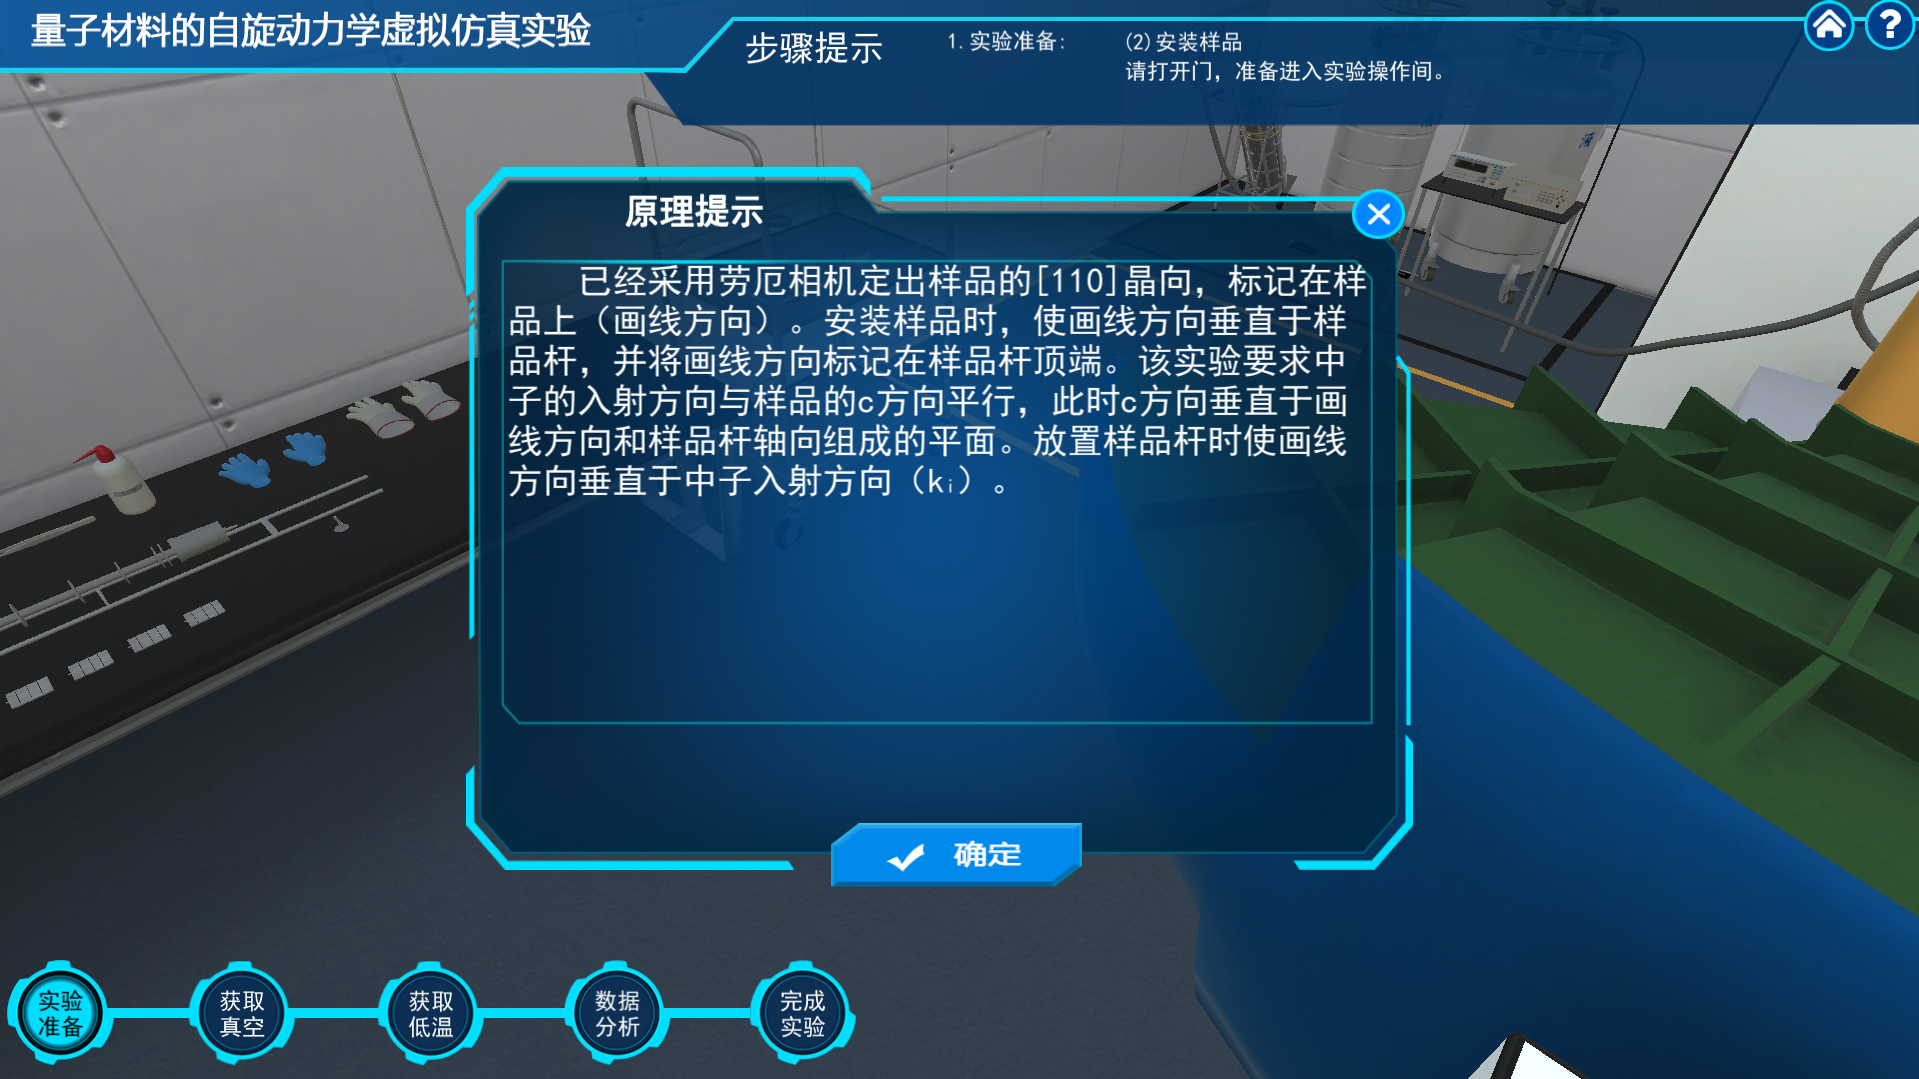
\includegraphics[width=\linewidth]{屏幕截图 2026-06-28 112549.png}
        \caption{自旋波测量原理提示}
    \end{subfigure}
    \hfill
    \begin{subfigure}[t]{0.48\textwidth}
        \centering
        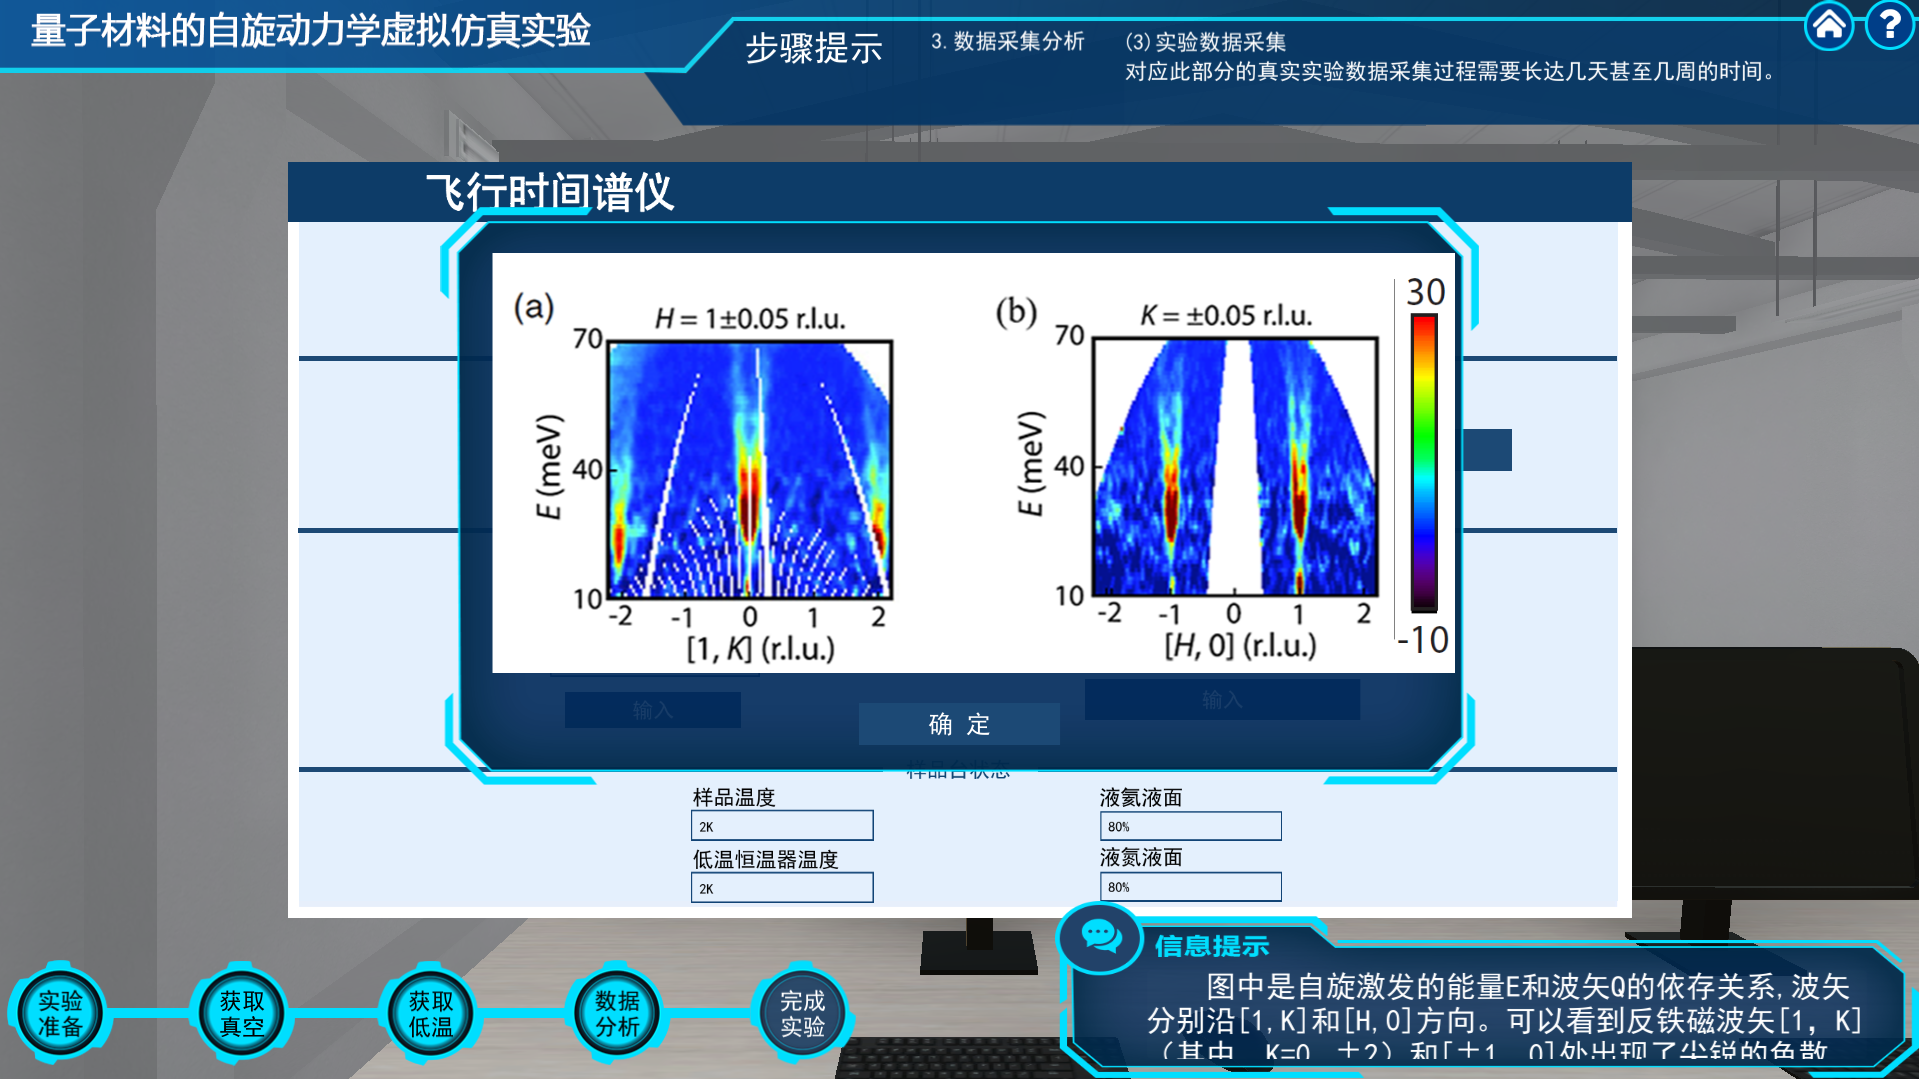
\includegraphics[width=\linewidth]{屏幕截图 2026-06-28 113128.png}
        \caption{平台给出的飞行时间谱参考图}
    \end{subfigure}
    \caption{BaFe$_2$As$_2$ 自旋波谱测量的实验准备}
    \label{fig:spin-preparation}
\end{figure}

\section{结果与分析}

\subsection{实验模块关系}

本虚拟实验的三个模块并不是彼此独立的操作演示，而是按照从概念到仪器、从声子到自旋激发的顺序递进。表 \ref{tab:modules} 总结了各模块的主要任务和物理意义。

\begin{table}[H]
    \centering
    \caption{虚拟仿真实验模块与主要认识}
    \label{tab:modules}
    \begin{tabular}{p{0.22\textwidth}p{0.36\textwidth}p{0.32\textwidth}}
        \toprule
        模块 & 实验任务 & 主要认识 \\
        \midrule
        预习与学习 & 学习量子材料、自旋动力学、中子谱仪、低温环境与辐射安全 & 明确中子散射适合同时研究结构、声子和磁激发 \\
        金刚石声子谱 & 利用三轴谱仪进行弹性散射定向，再进行非弹性能量扫描 & 建立仪器参数、倒易空间点和声子分支之间的联系 \\
        BaFe$_2$As$_2$ 自旋波谱 & 在低温磁有序态下利用飞行时间谱仪测量自旋激发 & 观察反铁磁波矢附近自旋波及其能量依赖性 \\
        \bottomrule
    \end{tabular}
\end{table}

其中，金刚石模块相当于谱学方法的基础训练：样品结构明确、声子分支清晰，便于理解弹性定向和非弹性扫描。BaFe$_2$As$_2$ 模块则把同样的谱学思想用于更复杂的量子材料磁激发，使实验重点从晶格振动扩展到自旋动力学。

\subsection{金刚石声子谱分析}

金刚石声子谱测量中，弹性散射定向是后续非弹性扫描的基础。若晶体取向和仪器角度之间的关系没有准确建立，之后设定的 $q$ 点就不能对应预期的高对称方向，声子分支的识别也会出现偏差。因此，实验先利用 Bragg 点确定散射面，再通过扫描峰位修正样品角。

在非弹性散射阶段，沿 $[4+q,0,0]$ 方向测得纵波分支，沿 $[4,q,0]$ 方向测得横波分支。金刚石沿 [100] 方向的声子谱可分辨四支主要分支：TA、LA、TO 和 LO。低能声学支对应晶胞整体平移型振动，光学支对应基元内部原子的相对振动，因此光学支能量明显高于声学支。

图 \ref{fig:phonon-peaks} 给出了四类声子分支的代表性扫描结果。各扫描曲线均出现清晰的单峰结构，红色拟合曲线与绿色数据点符合较好，可据此读出相应 $q$ 点的峰值能量。纵波与横波采用不同的倒易空间扫描方向，因此能够分别提取 LA、LO 与 TA、TO 分支。

\begin{figure}[H]
    \centering
    \begin{subfigure}[t]{0.48\textwidth}
        \centering
        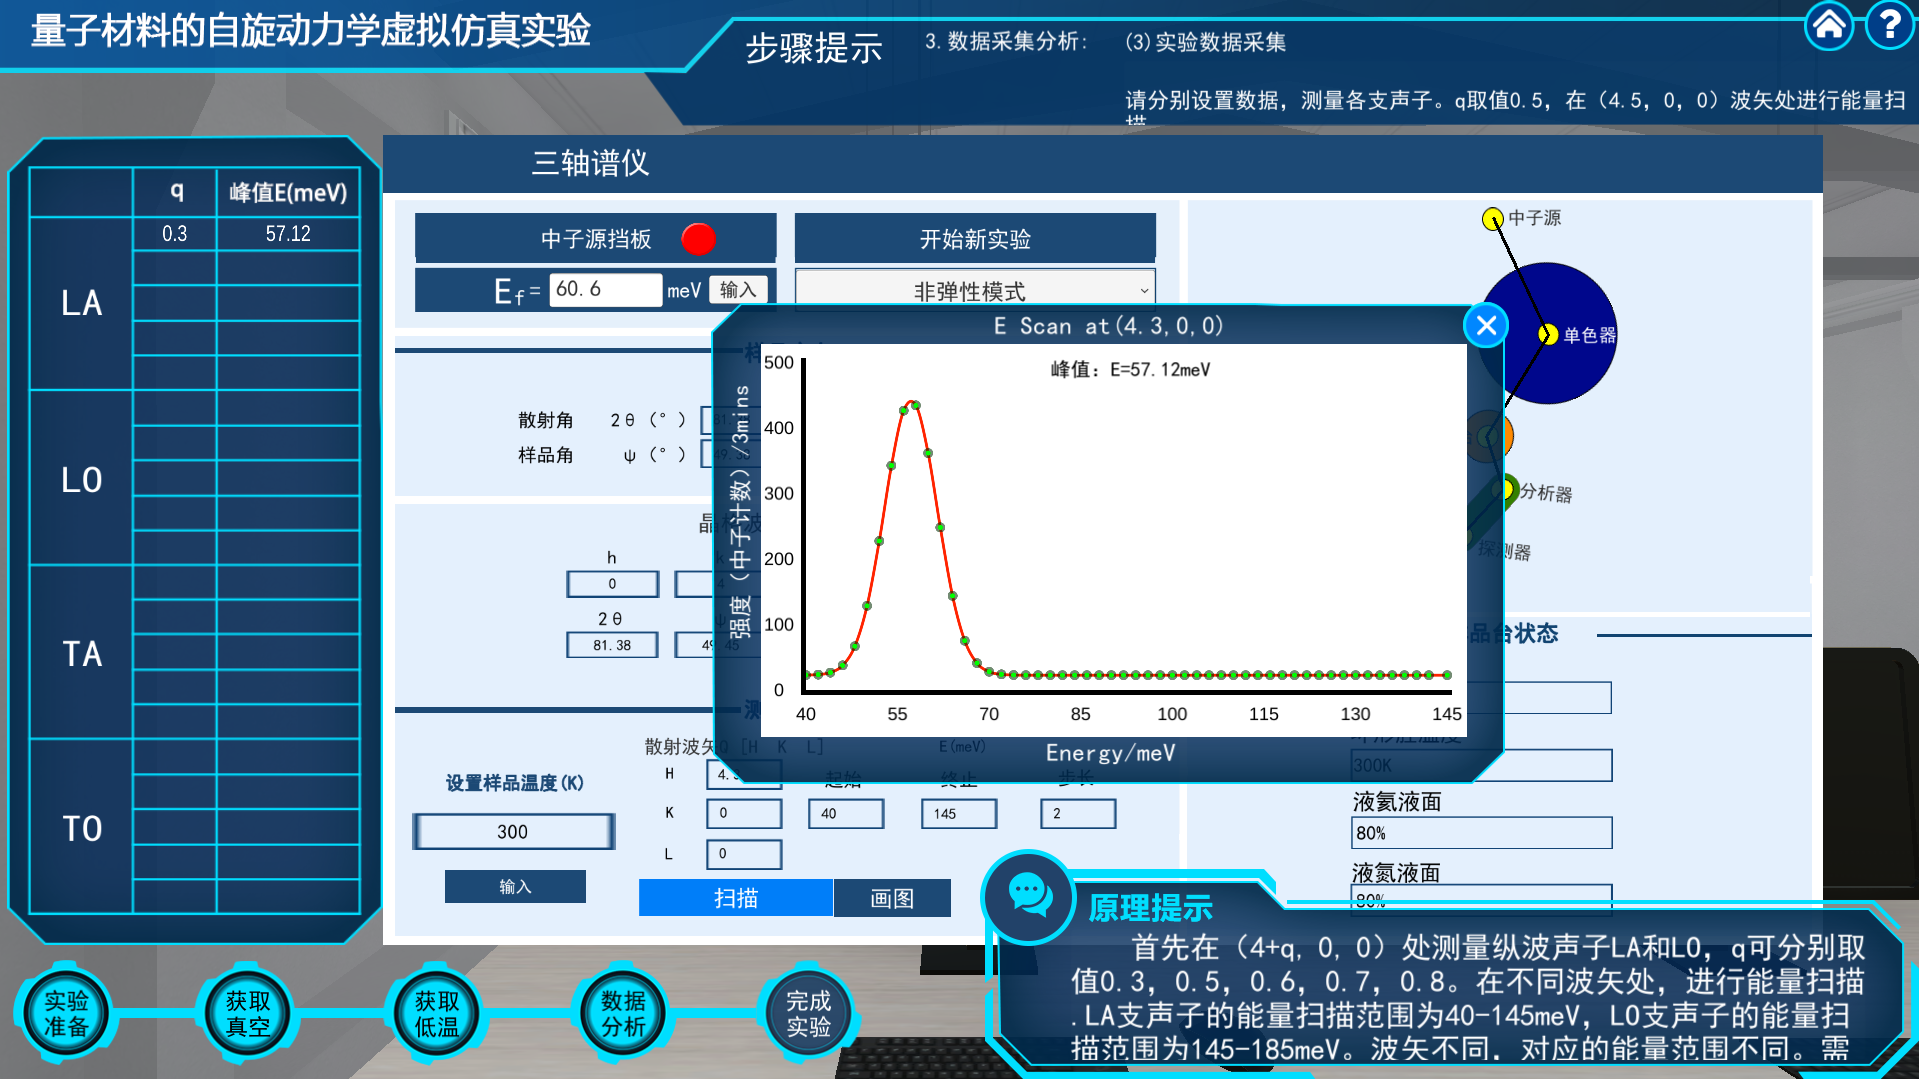
\includegraphics[width=\linewidth]{屏幕截图 2026-06-28 111049.png}
        \caption{LA 支：$q=0.3$}
    \end{subfigure}
    \hfill
    \begin{subfigure}[t]{0.48\textwidth}
        \centering
        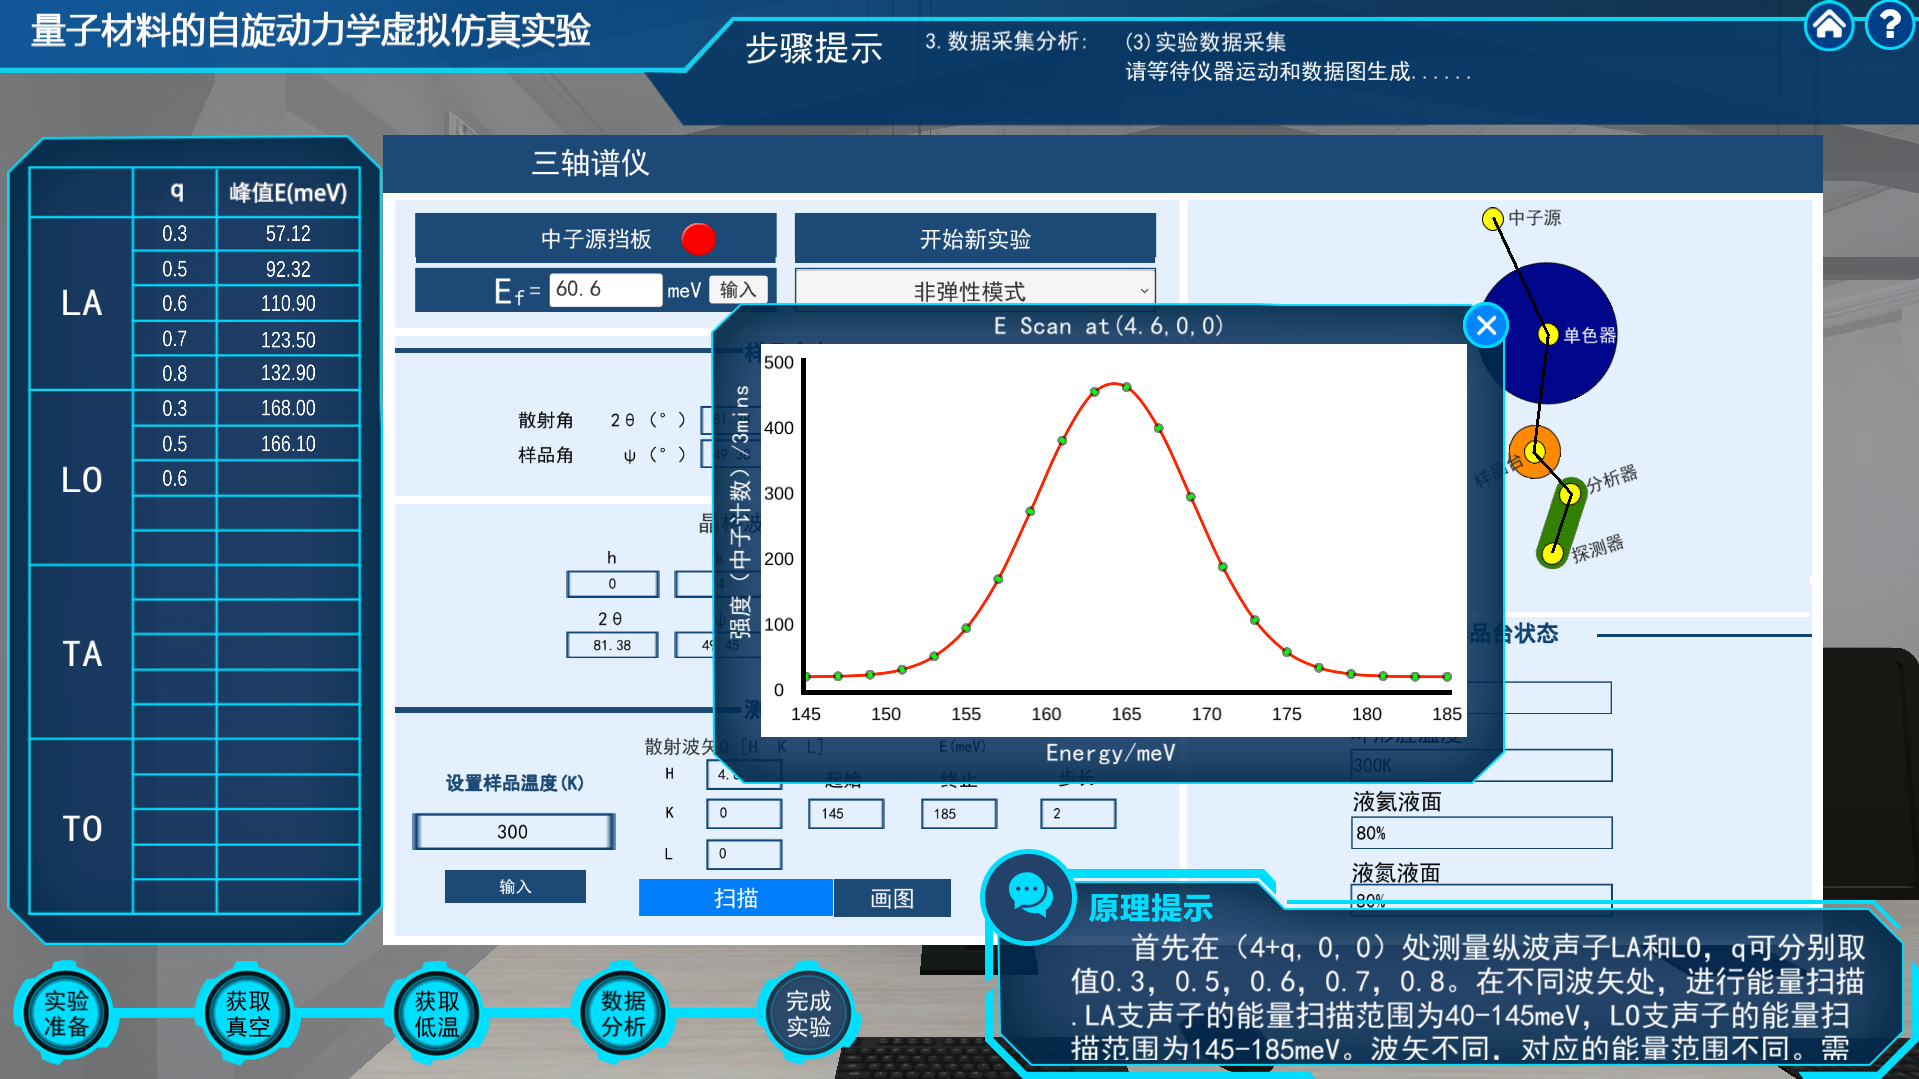
\includegraphics[width=\linewidth]{屏幕截图 2026-06-28 111307.png}
        \caption{LO 支：$q=0.6$}
    \end{subfigure}

    \vspace{0.5em}
    \begin{subfigure}[t]{0.48\textwidth}
        \centering
        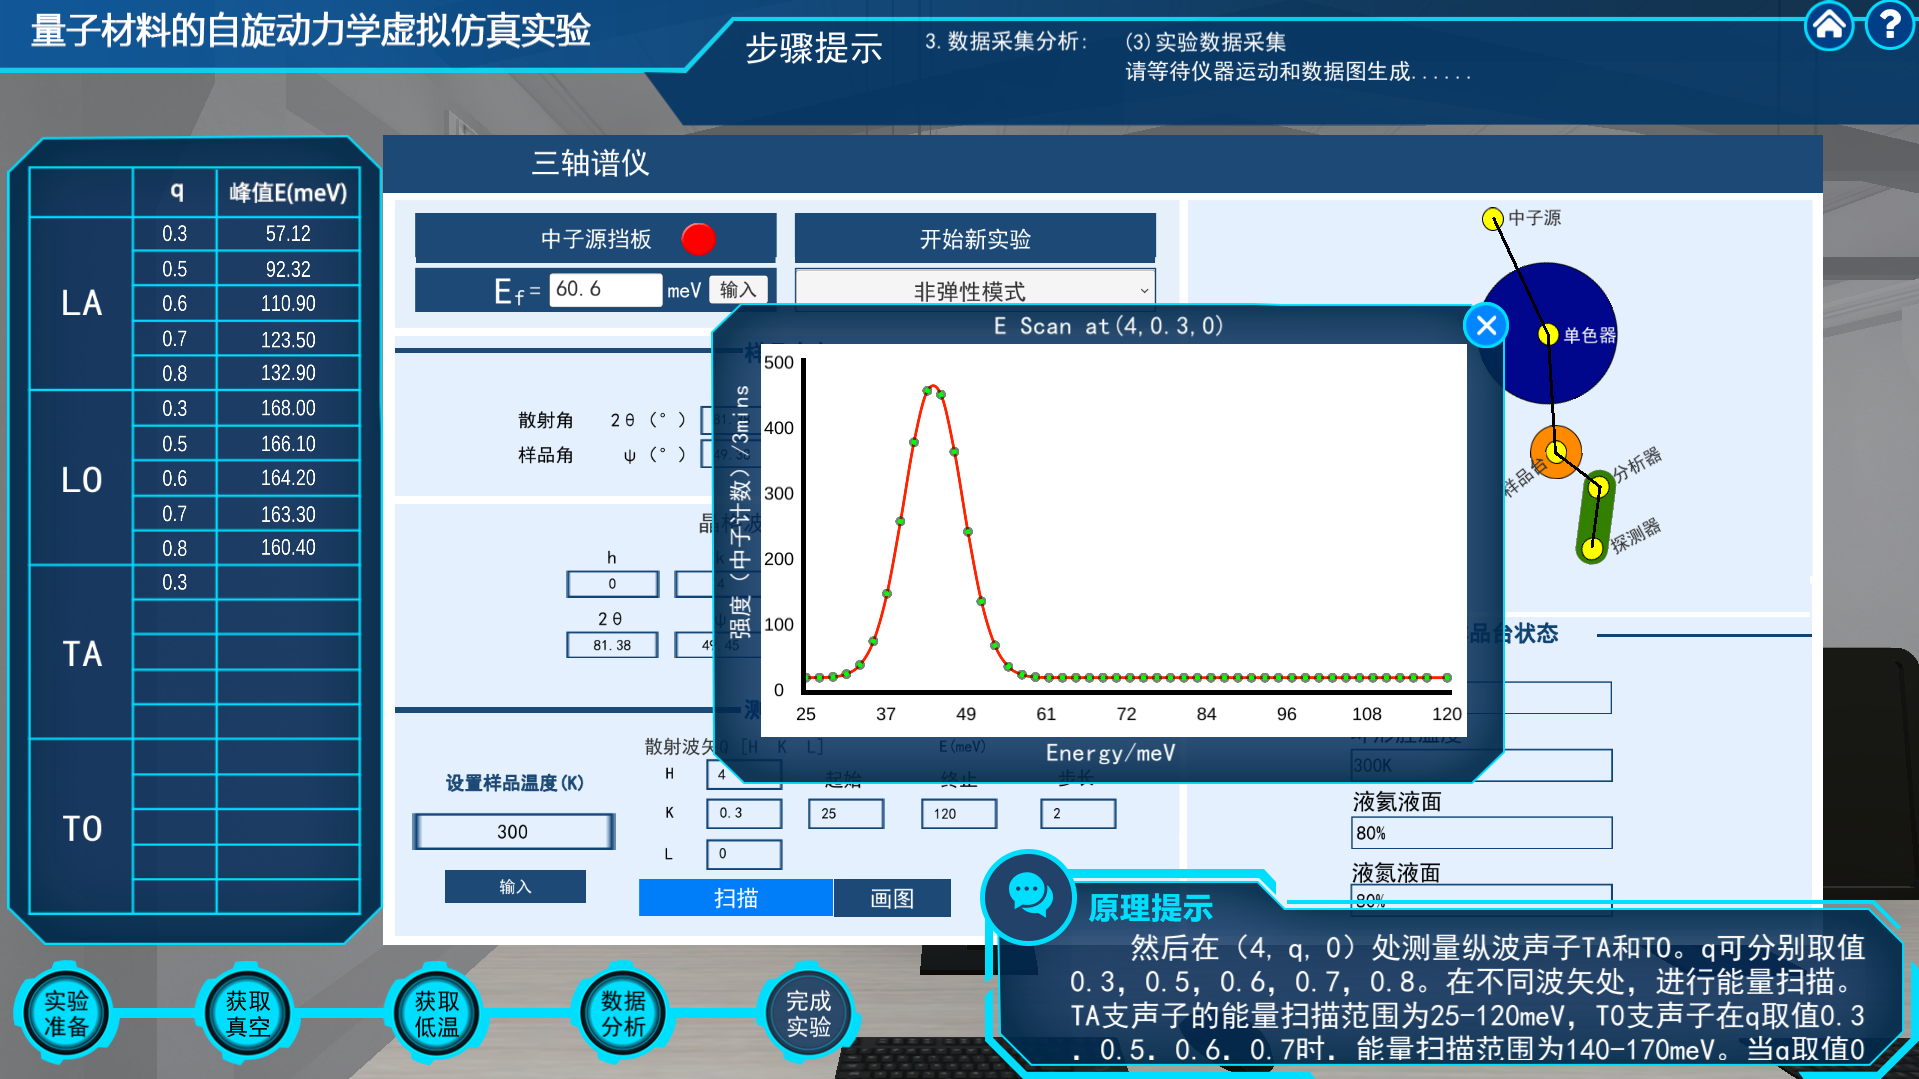
\includegraphics[width=\linewidth]{屏幕截图 2026-06-28 111409.png}
        \caption{TA 支：$q=0.3$}
    \end{subfigure}
    \hfill
    \begin{subfigure}[t]{0.48\textwidth}
        \centering
        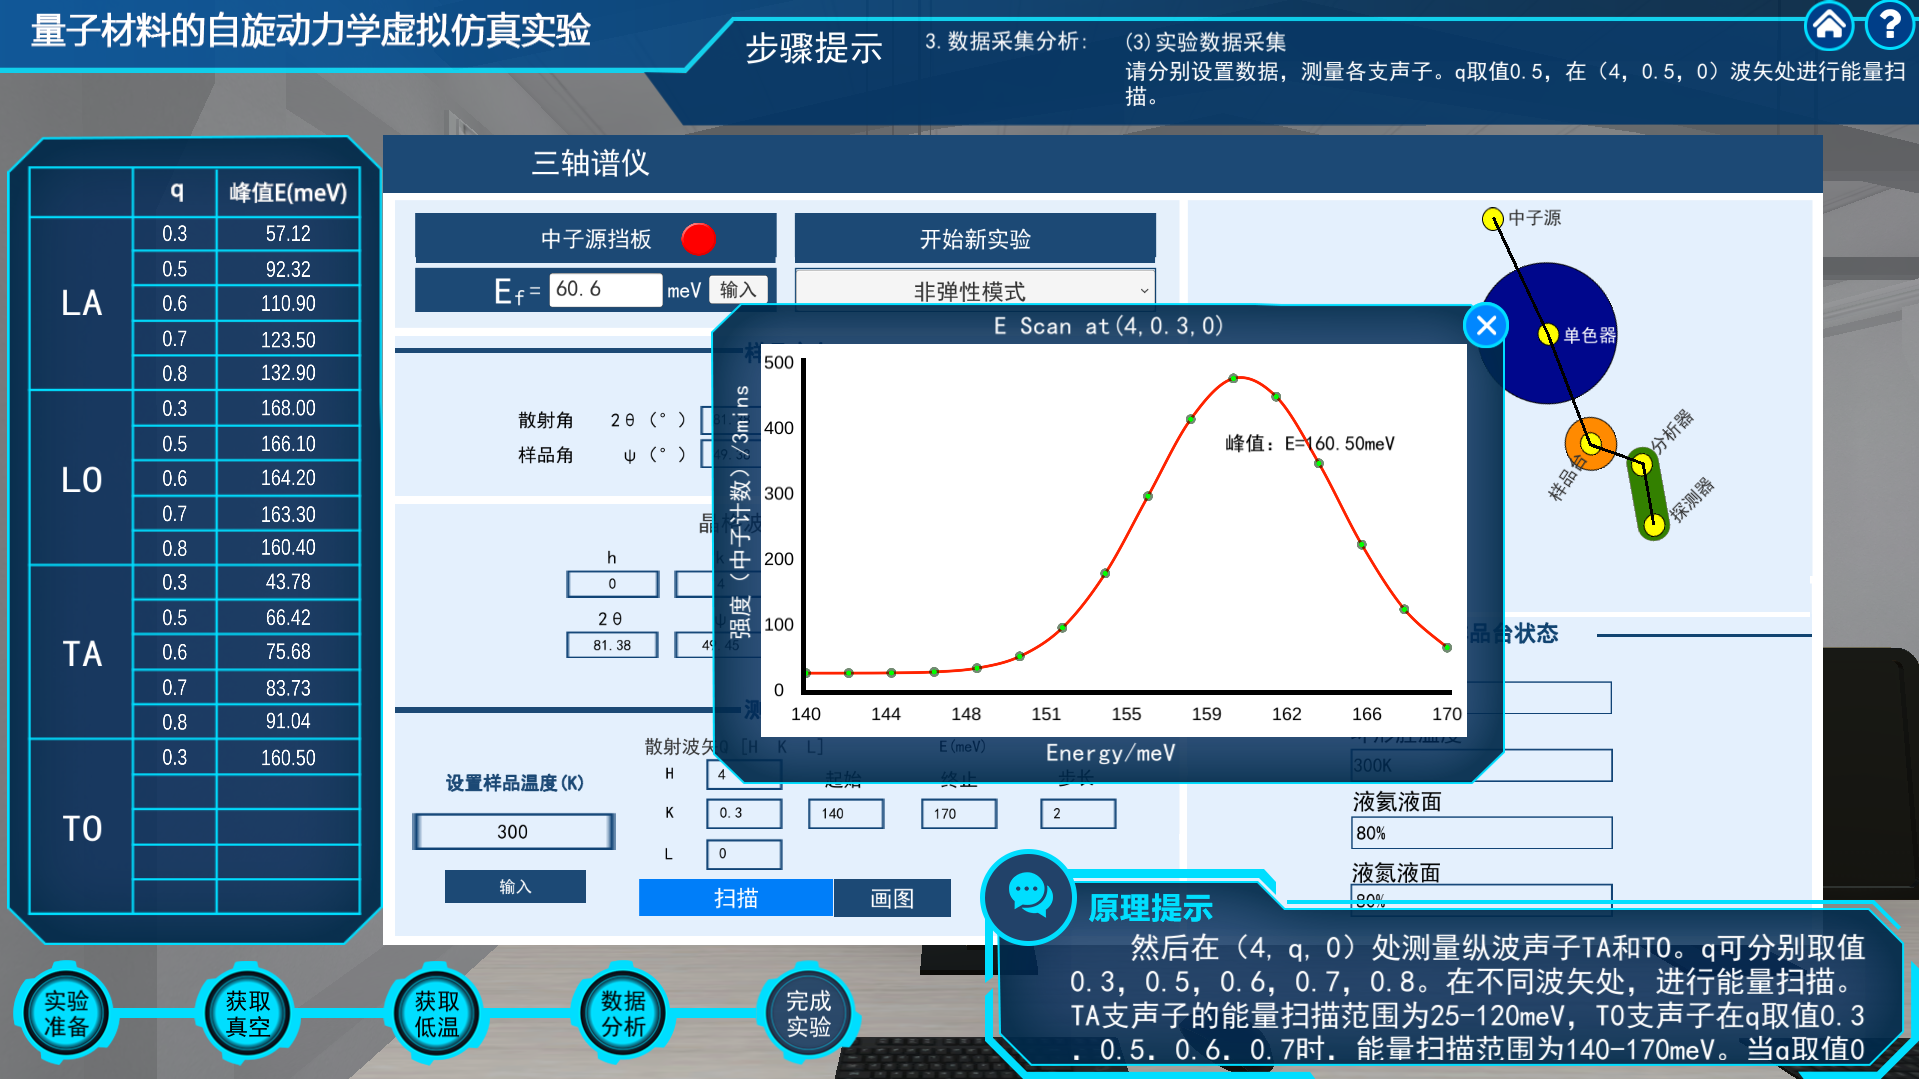
\includegraphics[width=\linewidth]{屏幕截图 2026-06-28 111606.png}
        \caption{TO 支：$q=0.3$}
    \end{subfigure}
    \caption{四类声子分支的代表性能量扫描曲线}
    \label{fig:phonon-peaks}
\end{figure}

逐点读取所有扫描峰位后，得到表 \ref{tab:phonon-data} 所列实验数据。LA 和 TA 支能量随 $q$ 增大而上升，其中 LA 支的上升更快；LO 和 TO 支总体随 $q$ 增大而下降，且 LO 支变化较缓。这些数据共同构成图 \ref{fig:phonon-dispersion} 所示的金刚石 [100] 方向声子色散。

\begin{table}[H]
    \centering
    \caption{金刚石沿 [100] 方向各声子分支的峰值能量}
    \label{tab:phonon-data}
    \small
    \begin{tabular}{ccccc}
        \toprule
        $q$ & $E_{\mathrm{LA}}$ (meV) & $E_{\mathrm{LO}}$ (meV) &
        $E_{\mathrm{TA}}$ (meV) & $E_{\mathrm{TO}}$ (meV) \\
        \midrule
        0.3 & 57.12 & 168.00 & 43.78 & 160.50 \\
        0.5 & 92.32 & 166.10 & 66.42 & 151.70 \\
        0.6 & 110.90 & 164.20 & 75.68 & 149.10 \\
        0.7 & 123.50 & 163.30 & 83.73 & 144.10 \\
        0.8 & 132.90 & 160.40 & 91.04 & 140.40 \\
        \bottomrule
    \end{tabular}
\end{table}

\begin{figure}[H]
    \centering
    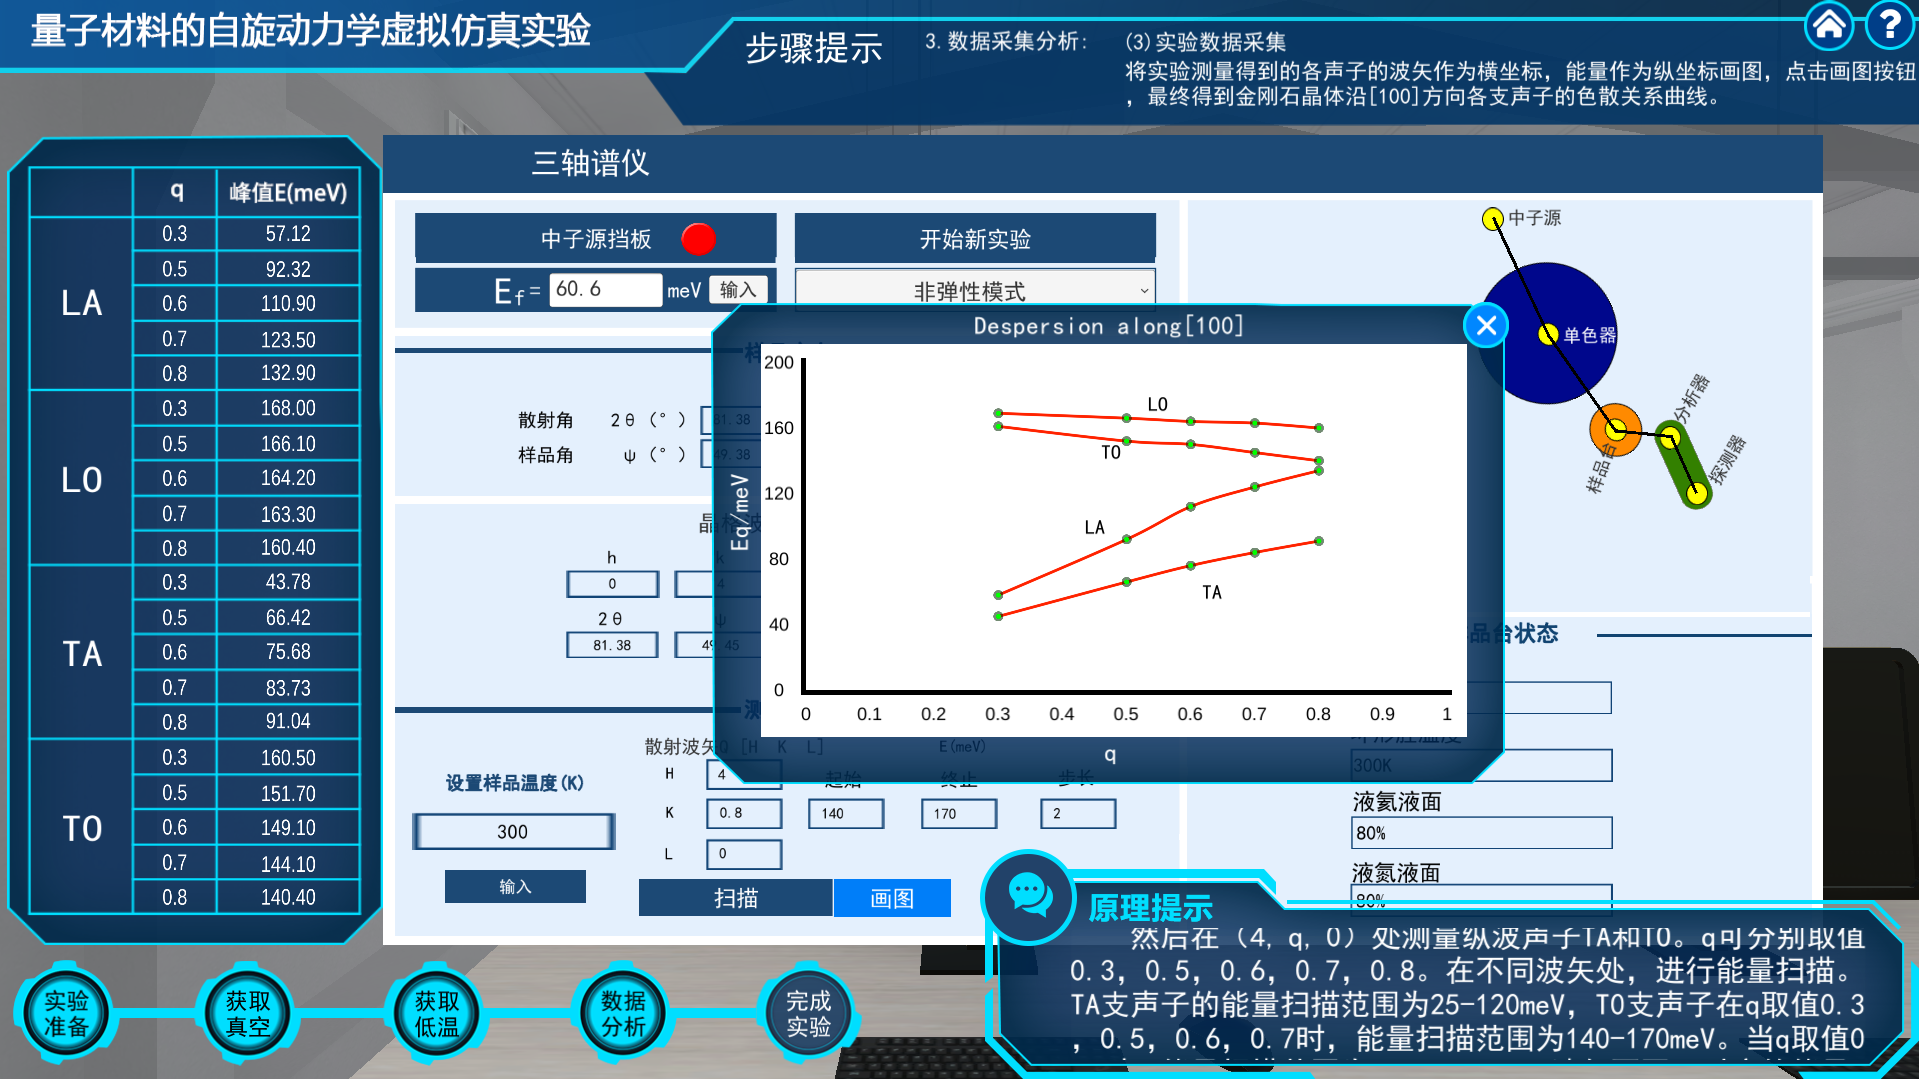
\includegraphics[width=0.9\textwidth]{屏幕截图 2026-06-28 111826.png}
    \caption{实验平台汇总得到的金刚石 [100] 方向声子色散关系}
    \label{fig:phonon-dispersion}
\end{figure}

从物理图像上看，声子谱不是单个峰的孤立测量，而是在倒易空间中沿给定方向逐点寻找激发峰位。不同 $q$ 点的峰值能量共同构成色散关系。这个过程体现了非弹性中子散射的核心逻辑：通过中子损失或获得的能量，反推出样品内部集体激发的能量尺度。

\subsection{BaFe$_2$As$_2$ 低能自旋激发}

BaFe$_2$As$_2$ 只有在低于磁相变温度后才形成稳定的反铁磁有序，因此低温条件是观察清晰自旋波信号的前提。在 $E=[58,64]\,\mathrm{meV}$ 的低能窗口中，谱图在反铁磁波矢附近出现强度集中区域，可理解为磁有序背景上的集体自旋激发。

低能谱图的分析需要同时关注坐标轴、能量积分窗口、颜色强度标尺和不可测区域。强度集中若位于预期反铁磁波矢附近，说明实验参数选择能够有效捕捉目标磁激发；若样品温度高于 $T_N$，长程磁有序被破坏，自旋波信号将显著减弱或变得难以辨认。因此，低能测量的主要意义在于确认自旋激发是否存在以及激发中心是否位于正确倒易空间位置。

\begin{figure}[H]
    \centering
    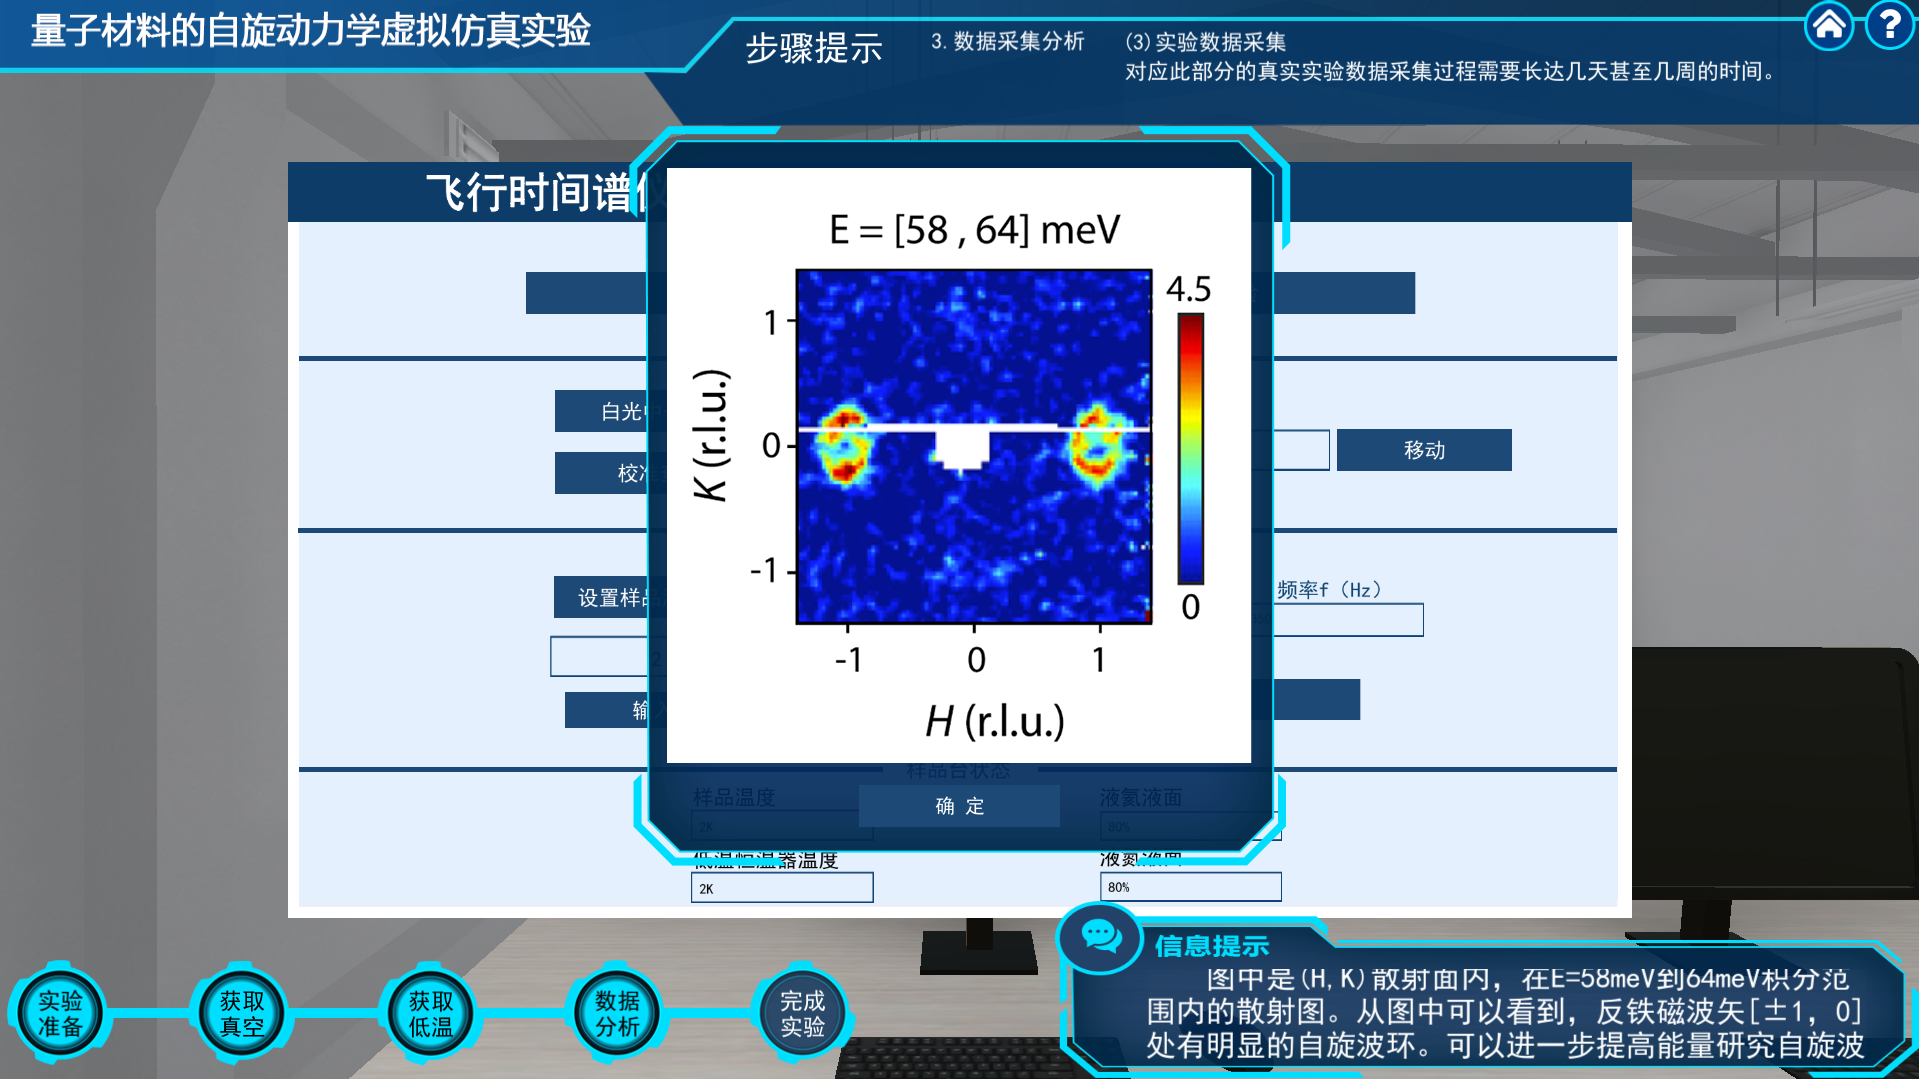
\includegraphics[width=0.88\textwidth]{屏幕截图 2026-06-28 113138.png}
    \caption{$E=[58,64]\,\mathrm{meV}$ 能量窗口内的低能自旋激发强度分布}
    \label{fig:spin-low}
\end{figure}

\subsection{BaFe$_2$As$_2$ 高能自旋激发}

提高入射能量后，飞行时间谱仪能够进入更高的能量转移范围。在 $E=[213,234]\,\mathrm{meV}$ 的高能窗口中，自旋激发的分布不再只是低能区中局域的强度集中，而表现出更明显的对称性和较大动量空间范围内的结构。

低能与高能结果结合说明，自旋激发具有显著的能量依赖性。低能图更适合确认反铁磁波矢附近的激发中心，高能图则更适合观察磁相互作用在较宽能量范围内留下的谱学特征。对于铁基超导母体材料而言，这种自旋激发与磁涨落、结构相变以及可能的超导配对机制密切相关，因此自旋动力学测量不仅是对磁有序的表征，也为理解材料的整体量子性质提供线索。

实验还记录了中间能量窗口 $E=[120,135]\,\mathrm{meV}$ 的强度图。由图 \ref{fig:spin-mid-high} 可见，随能量提高，低能区相对集中的激发逐渐向更大的动量范围扩展；到 $E=[213,234]\,\mathrm{meV}$ 时，强度分布呈现更复杂而近似对称的结构。这一变化直观体现了自旋波的色散特征。

\begin{figure}[H]
    \centering
    \begin{subfigure}[t]{0.48\textwidth}
        \centering
        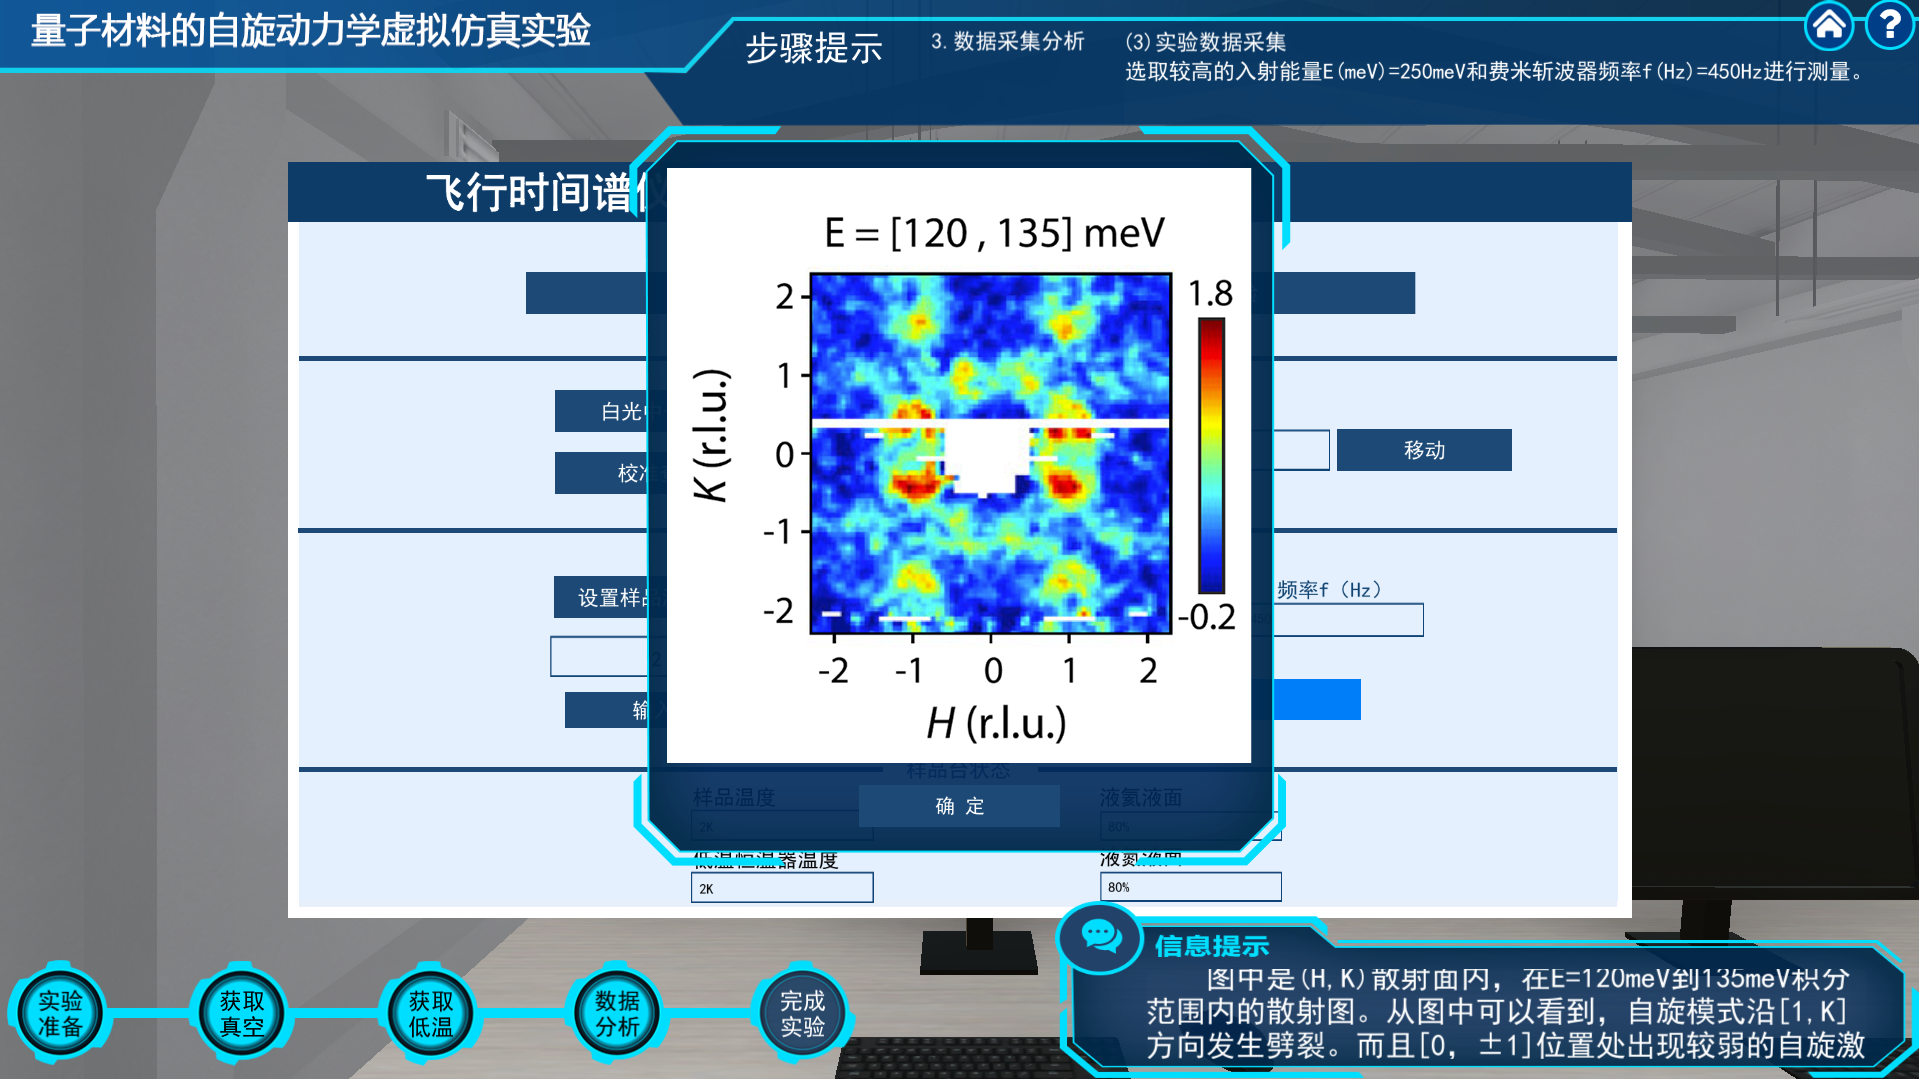
\includegraphics[width=\linewidth]{屏幕截图 2026-06-28 113154.png}
        \caption{$E=[120,135]\,\mathrm{meV}$}
    \end{subfigure}
    \hfill
    \begin{subfigure}[t]{0.48\textwidth}
        \centering
        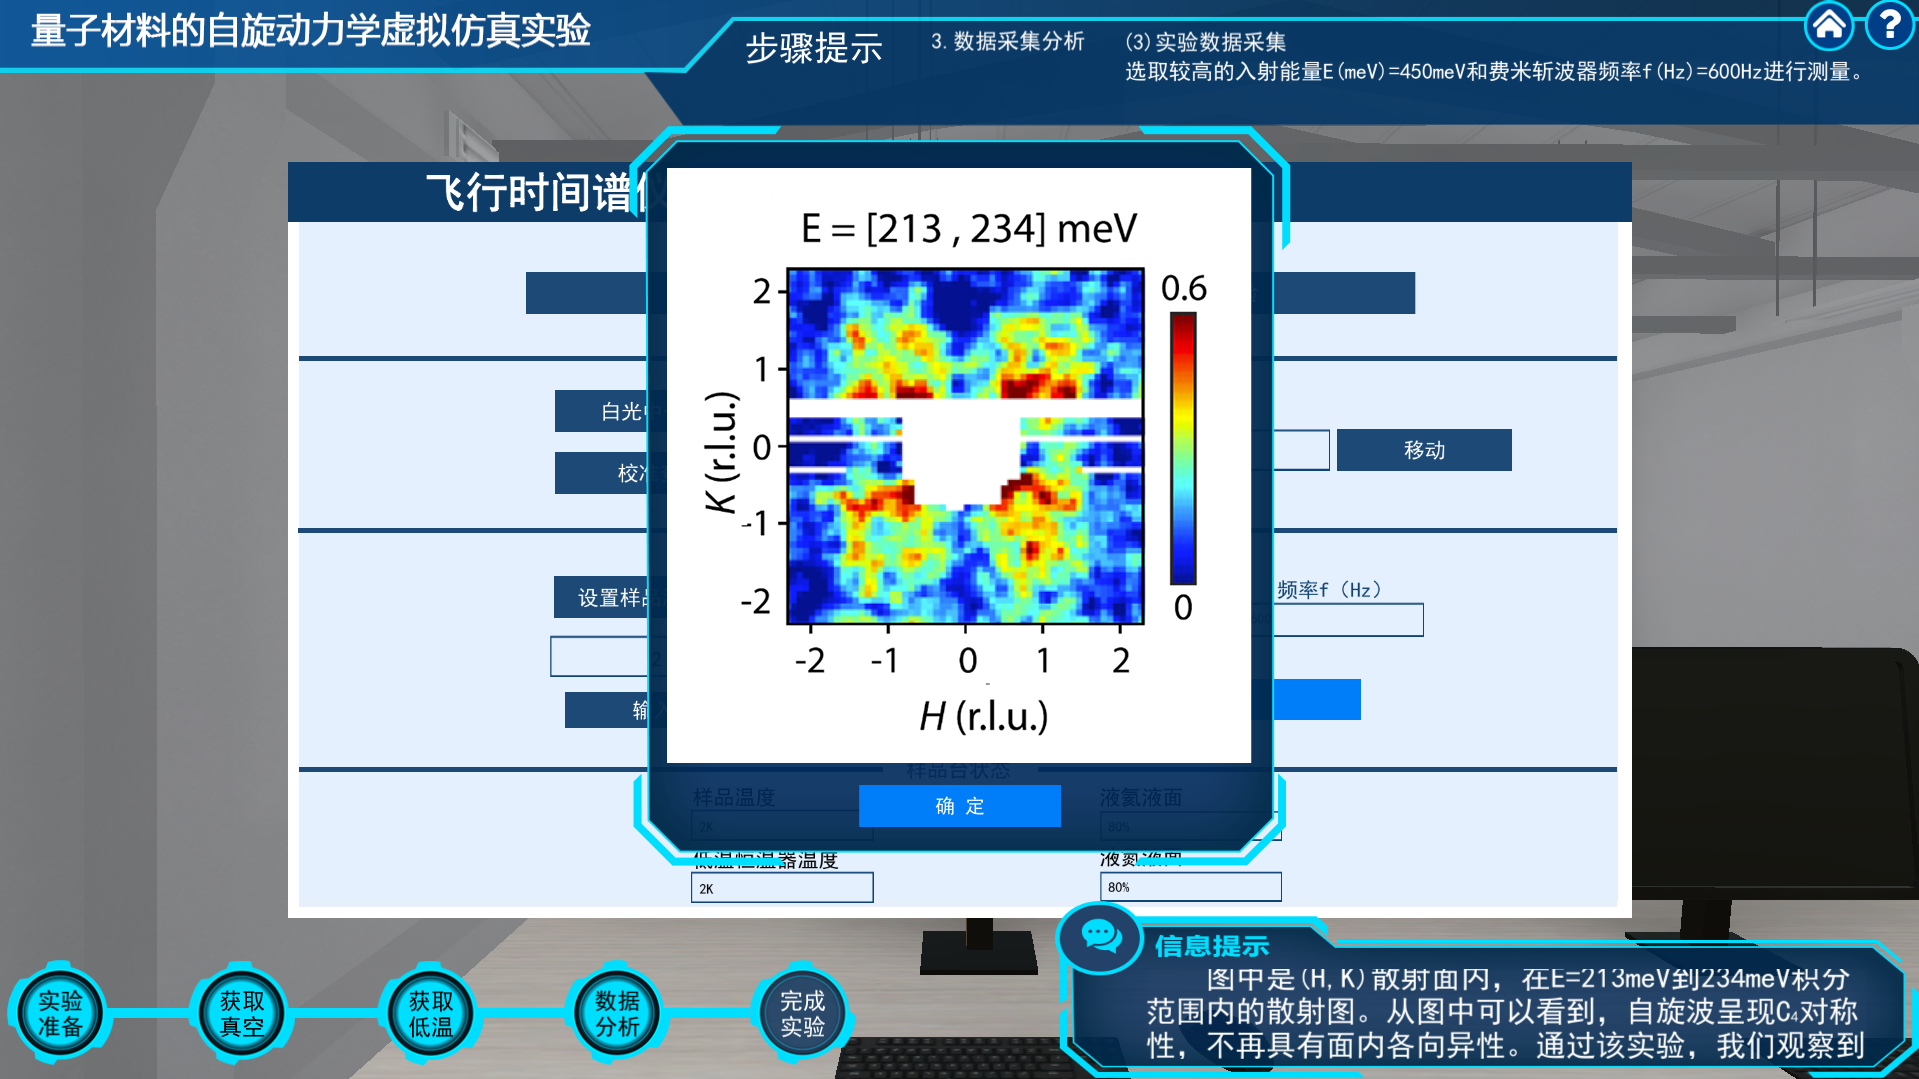
\includegraphics[width=\linewidth]{屏幕截图 2026-06-28 113208.png}
        \caption{$E=[213,234]\,\mathrm{meV}$}
    \end{subfigure}
    \caption{中、高能窗口内的自旋激发强度分布}
    \label{fig:spin-mid-high}
\end{figure}

\subsection{仪器方法比较}

三轴谱仪和飞行时间谱仪都可用于非弹性中子散射，但适用场景不同。三轴谱仪分辨率高，适合对指定 $\mathbf{Q}$ 点进行精细能量扫描；飞行时间谱仪覆盖范围大，适合快速获得二维或多维能量--动量谱图。表 \ref{tab:instrument} 给出二者的比较。

\begin{table}[H]
    \centering
    \caption{三轴谱仪与飞行时间谱仪的比较}
    \label{tab:instrument}
    \begin{tabular}{p{0.22\textwidth}p{0.33\textwidth}p{0.33\textwidth}}
        \toprule
        项目 & 三轴谱仪 & 飞行时间谱仪 \\
        \midrule
        测量方式 & 逐点选择 $\mathbf{Q}$ 和 $E$ & 一次测量覆盖较宽能量--动量空间 \\
        优点 & 分辨率高，适合精细扫描 & 覆盖范围大，适合寻找整体谱图 \\
        典型任务 & 样品定向、声子峰精细测量 & 自旋波整体分布、高能激发与各向异性 \\
        本实验应用 & 金刚石声子谱 & BaFe$_2$As$_2$ 自旋波谱 \\
        \bottomrule
    \end{tabular}
\end{table}

这种差异说明，实验仪器参数不是附属步骤，而会直接决定能够观察到的物理信息。对于未知材料，通常需要先用覆盖范围较大的方法寻找激发特征，再用高分辨方法进行局部精细测量。

\section{问题讨论}

\subsection{弹性散射与非弹性散射的作用}

弹性散射主要用于确定样品结构和取向。由于散射前后能量相同，峰位由晶格周期性决定，适合通过 Bragg 峰寻找倒易晶格方向。非弹性散射则关注中子与样品交换能量后的谱峰，能够反映声子、自旋波等动态激发。因此，在同一实验中，弹性散射通常服务于实验准备和样品定向，非弹性散射才是获取动力学信息的核心。

\subsection{低温和安全规范的意义}

本实验虽然是虚拟仿真，但低温、真空和辐射安全步骤并非形式化内容。对于 BaFe$_2$As$_2$，只有样品进入反铁磁有序态温区，才具备观察自旋波的物理前提；对于真实中子实验，真空隔热和液氦回收关系到温度稳定性与实验成本，辐射剂量检测则关系到人员安全。实验结束后升温至室温、关闭中子束挡板并检测剂量，体现了大型装置实验中“完成采集”并不等于“完成实验”的规范意识。

\subsection{虚拟仿真实验的价值与局限}

中子散射实验依赖大型装置，真实束流时间有限，操作成本高，且涉及低温和辐射安全要求。虚拟仿真实验能够把复杂实验拆解为可重复练习的模块，使学生在不接触真实危险源的情况下理解仪器逻辑和数据分析方法。其局限在于无法完全替代真实实验中的调束、对准、统计涨落和设备响应等操作体验。因此，虚拟实验更适合作为进入真实大型装置实验前的概念训练和流程预演。

\section{结论}

本次虚拟仿真实验完成了预习与学习、金刚石声子谱测量和 BaFe$_2$As$_2$ 自旋波谱测量三个核心模块。实验表明，中子散射能够通过动量转移和能量转移同时表征晶体结构、晶格振动和磁激发，是研究量子材料动力学性质的重要手段。

在金刚石声子谱模块中，先利用弹性散射完成样品定向，再通过非弹性能量扫描得到沿 [100] 高对称方向的 TA、LA、TO、LO 四支主要声子分支，说明三轴谱仪适合高分辨逐点扫描。在 BaFe$_2$As$_2$ 自旋波谱模块中，样品被置于低于 $T_S\approx138\,\mathrm{K}$ 和 $T_N\approx137\,\mathrm{K}$ 的磁有序态温区，飞行时间谱仪在低能窗口 $E=[58,64]\,\mathrm{meV}$ 和高能窗口 $E=[213,234]\,\mathrm{meV}$ 中分别显示出自旋激发的中心位置、对称性和能量依赖性。

通过本实验，我进一步认识到，谱学实验的关键不仅是获得彩图或峰值，而是理解实验条件、仪器参数、倒易空间坐标和物理结论之间的对应关系。低温、真空、液氦系统和辐射防护也是中子散射实验不可分割的组成部分。总体而言，本实验帮助我从教材中的声子和自旋波概念过渡到按实验流程理解这些激发如何被实际测量出来。

\section{实验成绩}

虚拟仿真实验平台记录本次实验用时为 2 小时 29 分 8 秒，最终得分为 90 分，说明各实验模块及主要操作流程均已完成。平台成绩记录如图 \ref{fig:score} 所示。

\begin{figure}[H]
    \centering
    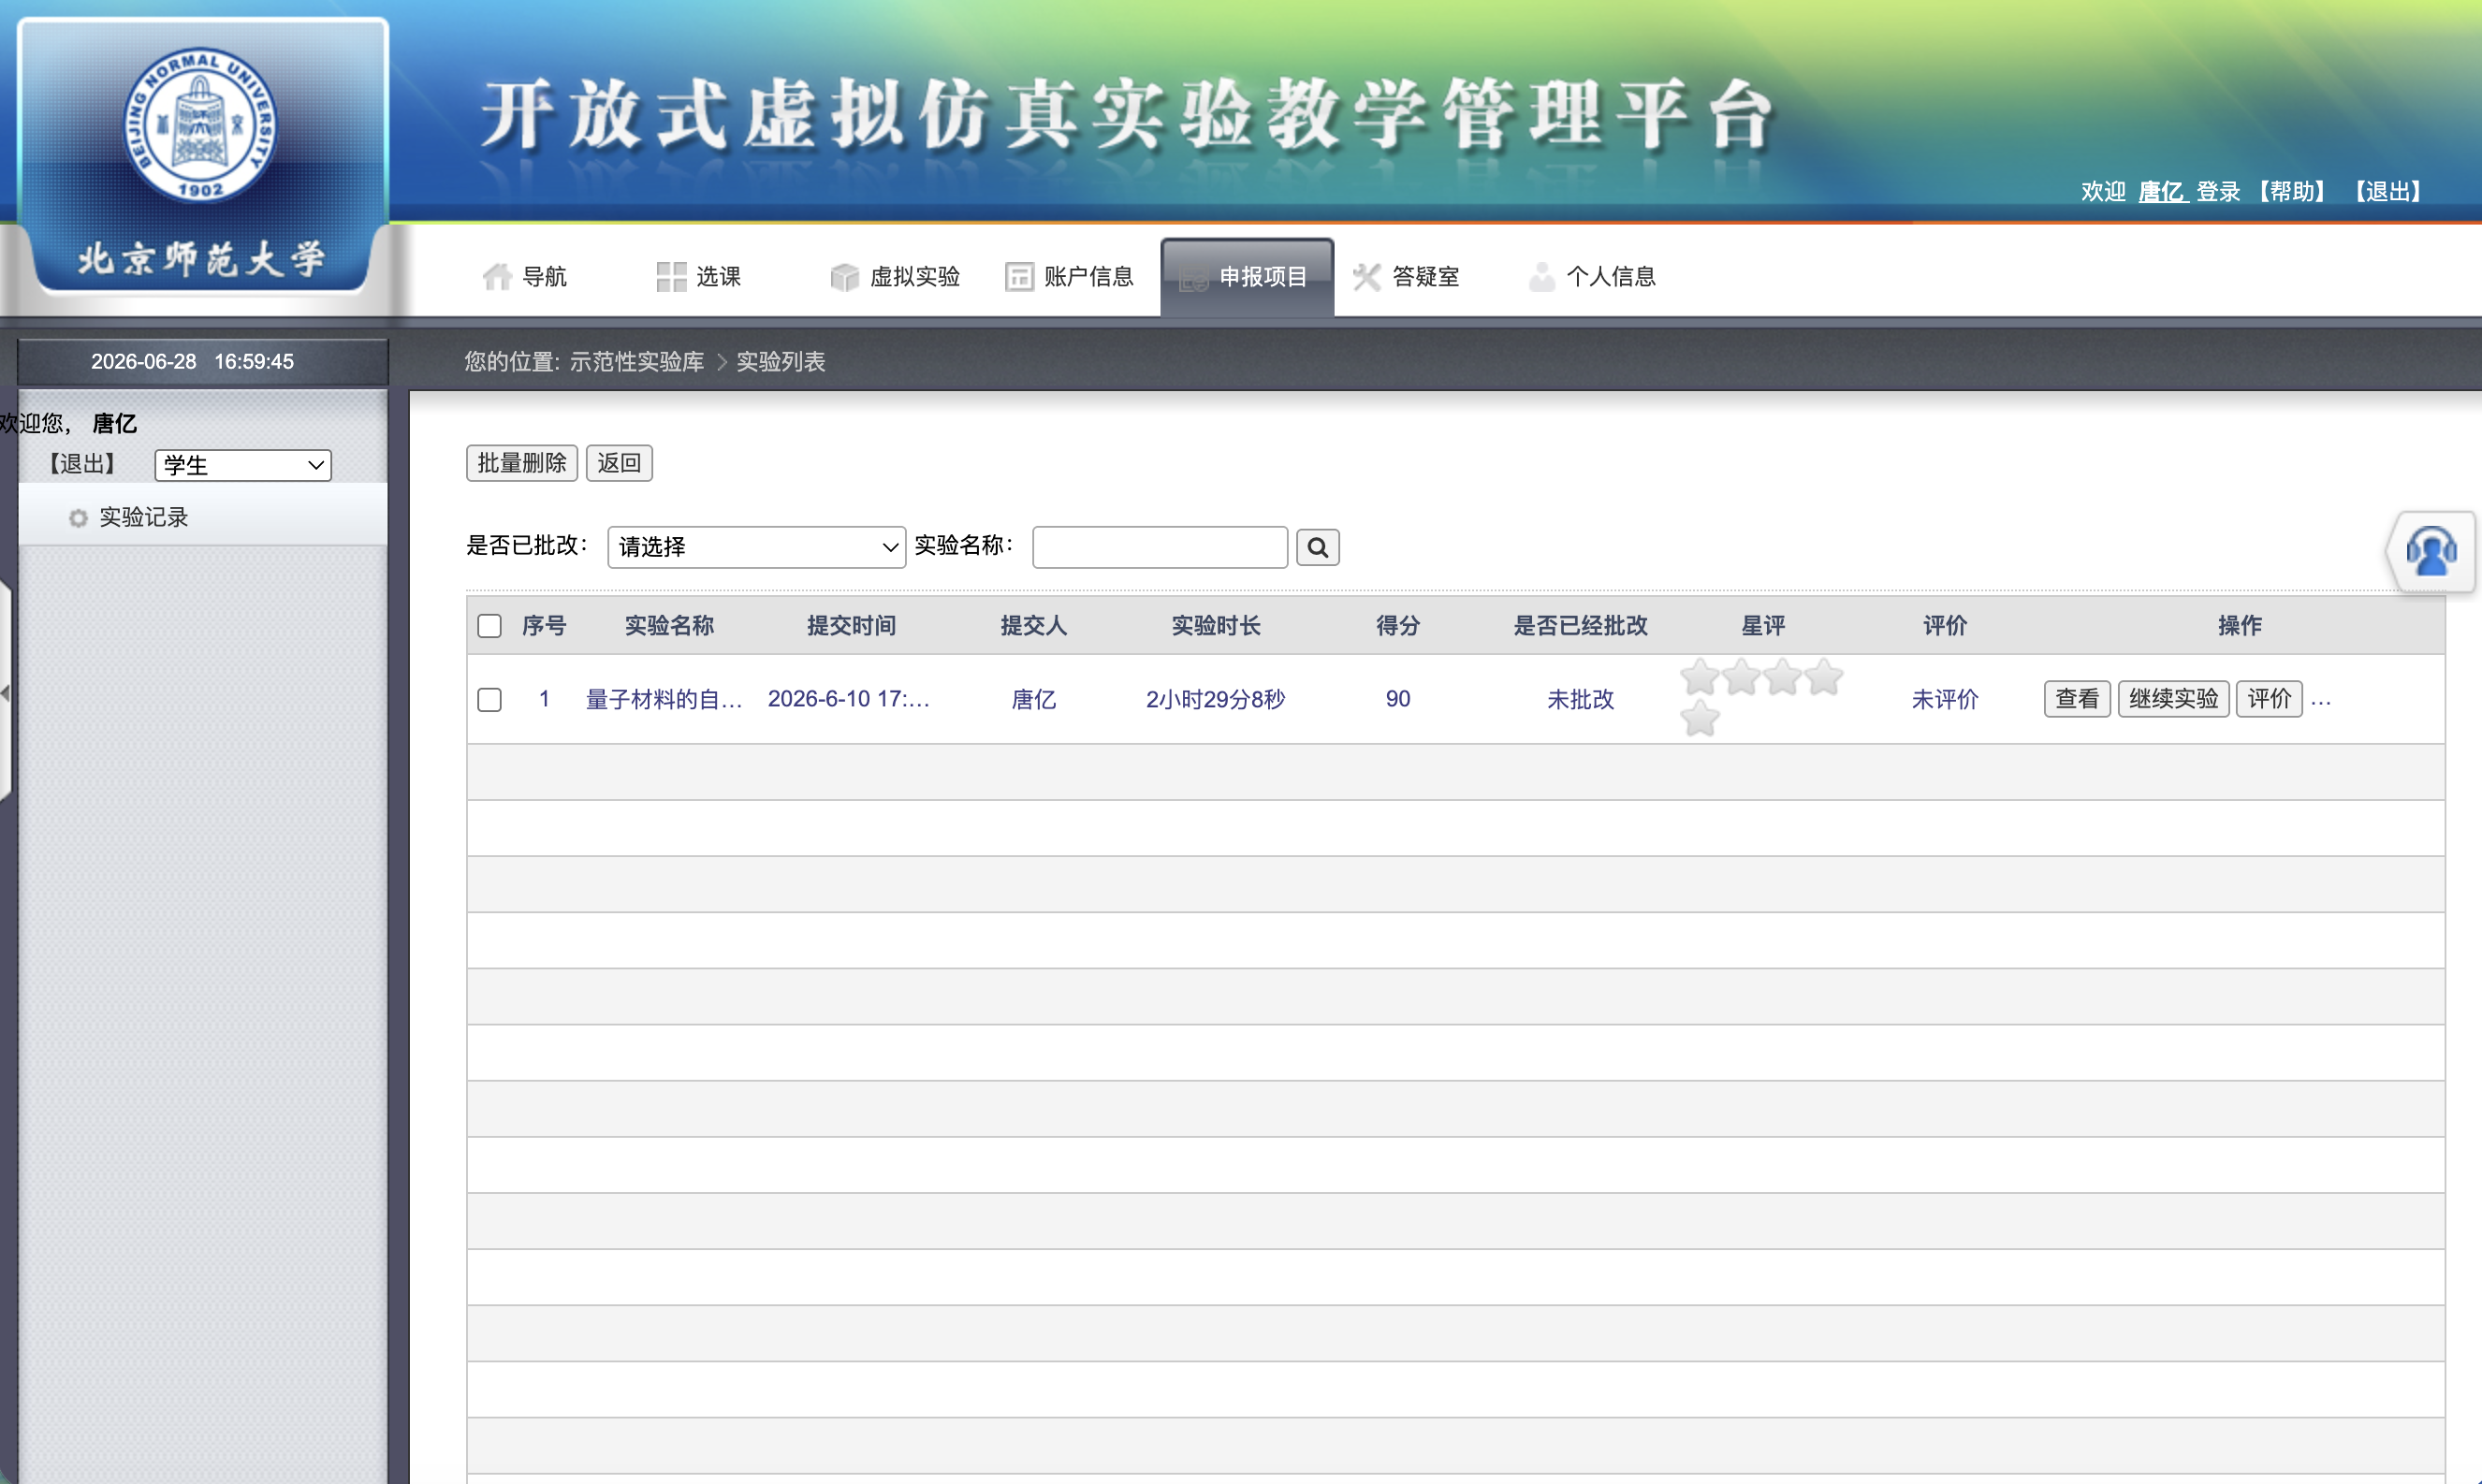
\includegraphics[width=\textwidth,trim=0 200 0 0,clip]{成绩截图.png}
    \caption{虚拟仿真实验平台成绩记录}
    \label{fig:score}
\end{figure}

\end{document}
